%		For public use only, fair use laws still apply
%		A tutorial template created by Chad Gibbons




%	I recommend for generic help the following website
%	http://www.emerson.emory.edu/services/latex/latex_toc.html
%	There are many good websites and forums for LaTeX
%
%	If you have a problem, google it. (ex. "How do I start my page numbers at a different number")



%%%%%%%%%%%%%%%%%%%%%%%%%%%%%%%%%%%%%%%%%%%%%%%%%%%%%%
%					 													  %
%					 													  %
%					  ALWAYS BEGIN THE PROGRAM WITH								  %
%					 													  %
%						\documentclass{class_type}								  %
%																		  %
%		Different class types have different commands associated with them, similar to header files			  %
%					 													  %
%					 													  %`
%%%%%%%%%%%%%%%%%%%%%%%%%%%%%%%%%%%%%%%%%%%%%%%%%%%%%%

\documentclass[12pt]{article}

%%%%%%%%%%%%%%%%%%%%%%%%%%%%%%%%%%%%%%%%%%%%%%%%%%%%%%
%					 													  %
%					 													  %
%				It is recommended to only use packages as you need them 						  %
%					 													  %
%	Different types of reports will consistently use specific packages; keep these in their respective templates		  %
%					 													  %
%					 													  %
%%%%%%%%%%%%%%%%%%%%%%%%%%%%%%%%%%%%%%%%%%%%%%%%%%%%%%


%\usepackage[a4paper,total={8.27in,11.69in},left=0.56in,right=0.56in,top=0.75in,bottom=1.69in]{geometry}		% 	Margins IEEE Articles
\usepackage[letterpaper,total={8.5in,11in},left=1.25in,top=1in,bottom=1in,right=1in]{geometry}		% 	Margins PDD
%\usepackage[a4paper,total={6.5in,9.375in}]{geometry}		% 	Margins MLA
%\usepackage{babel}				%	Expands text mode
\usepackage[english]{babel}
\usepackage{csquotes}				%	Permits \enquote{quote}
\usepackage{graphicx}				%	Permits \includegraphics[]{image}
\usepackage{caption}				%	Permits the void caption \caption*{}
\usepackage{titlesec}				%	Modify section titles
\usepackage{wrapfig}				% 	Insert wrappable objects like figures or tables
%\usepackage{a4wide}				% 	Expand width of body lazily
\usepackage{multicol}				% 	Permits multicolumn
\usepackage{multirow}				%	Permites utilization of multiple rows of a table
\usepackage{tocloft}				%	Permits modification of Table of Contents
\usepackage{amssymb}				%	Greek Alphabet Symbols
\usepackage{appendix}

\usepackage{scrextend}				% 	Permits padding margins of document


\graphicspath{ {./images/} }			%	Sets filepath to images folder in location of TeX Document

\usepackage[utf8]{inputenc}			%	biblatex depends on on this package
\usepackage{comment}
\usepackage[backend=bibtex,style=numeric]{biblatex}	%	LaTeX blibliography	%% Note: ieee stle lower-cases titles past first letter (Which seems wrong)
\bibliography{PDD_Draft}

%\addbibresource{hec2.bib}


			%	Makes Table of Contents Functionally a table of Hyperlinks
\usepackage{hyperref}
\hypersetup{
	colorlinks,
	citecolor= black,
	filecolor = black,
	linkcolor = blue,
	urlcolor = blue
	}

			%	Next Three Lines permit use of .tif images in \includegraphics
\usepackage{epstopdf}
\epstopdfDeclareGraphicsRule{.tif}{png}{.png}{convert #1 \OutputFile}
\AppendGraphicsExtensions{.tif}

\renewcommand{\thesection}{\Roman{section}} 
\renewcommand{\thesubsection}{\thesection.\Alph{subsection}}
\renewcommand{\thesubsubsection}{\thesection.\arabic{subsubsection}}
\setlength\cftsecnumwidth{3em}
\setlength\cftsubsecnumwidth{3em}
\setlength\cftsubsubsecnumwidth{3em}

			%	Define Abstract to be IEEE compliant (10pt, centered, roman numerals, capitalized)
\titleformat{\abstract}{\normalfont\btshape}{\Roman{section}}{1em}{\MakeUppercase}
			%	Define Sections to be IEEE compliant (10pt, centered, roman numerals, capitalized)
\titleformat{\section}{\normalfont\filcenter}{\Roman{section}.}{1em}{\MakeUppercase}
			%	Define Subections to be IEEE compliant (10pt, left, roman numerals, capitalized)
\titleformat{\subsection}{\normalfont\itshape}{\Alph{subsection}.}{1em}{}
			%	Define Subsubections to be IEEE compliant (10pt, left, roman numerals, capitalized, inline text)
\titleformat{\subsubsection}[runin]{\normalfont\itshape}{\indent\arabic{subsubsection}.)}{1em}{}
			%	Define Table of Contents to be IEEE compliant


			%	Next Two Lines Make Document San-Serif
%\renewcommand{\familydefault}{\sfdefault}		
%\usepackage{helvet}


\usepackage{textcomp}				%	For subsection symbol w/ \textsection
\usepackage{pdfpages}				%	For inserting PDF document and pages into LaTeX file
							%% 		Recommended pdfpages format : 									%%
							%%		\includepdf[pages=-,width=0.9\linewidth,pagecommand={}]{./appendices/file.pdf}		%%


%%%%%%%%%%%%%%%%%%%%%%%%%%%%%%%%%%%%%%%%%%%%%%%%%%%%%%%			PREAMBLE


\title{\Large \textbf{The University of Texas at Tyler\\
College of Engineering and Computer Science\\
Tyler, TX 75799\\
\hfill \\
\hfill \\[0.5em]
Primary Design Document Draft \\ For\\[0.5em]
Wireless Charger Project}}		%note left quote command vs " = \textquotedblright
%%  FIX FONT of Sub Sub Title  >> It should fit in with the text below. <<
\author{\large \hfill \\[0.5em] \textbf{A design project to fulfill the requirements of Senior Design}\\ \textbf{ 
in the Department of Electrical Engineering}\\ \textbf{ 
at The University of Texas at Tyler
}\hfill \\ \hfill \\[0.5em]}
\date{\normalsize \flushleft  The  individuals  whose  names  and  signatures  appear  below  certify  that  the  narrative, diagrams,  figures,  tables,  calculations,  and  analyses  contained  within  this  document  are their original work except as otherwise cited.
\hfill \\ \hfill \\[0.5em]
\underline{Flory, David\space\space\space\space\space\space\space\space\space\space\space} \hspace{0.25in}
\underline{\space\space\space\space\space\space\space\space\space\space\space\space\space\space\space\space\space\space\space\space\space\space\space\space\space\space\space\space\space\space\space\space\space\space\space\space\space\space\space\space\space} \hspace{0.25in}
\underline{\today \space\space\space\space\space\space\space} \hspace{0.25in}\\
\hspace{1.8in} Signature \hspace{1.8in} Date \hfill \\ \hfill \\
\underline{Franca, Natasha\space\space\space\space\space\space} \hspace{0.25in}
\underline{\space\space\space\space\space\space\space\space\space\space\space\space\space\space\space\space\space\space\space\space\space\space\space\space\space\space\space\space\space\space\space\space\space\space\space\space\space\space\space\space\space} \hspace{0.25in}
\underline{\today \space\space\space\space\space\space\space} \hspace{0.25in}\\
\hspace{1.8in} Signature \hspace{1.8in} Date \hfill \\ \hfill \\
\underline{Franulovic, Franci \space\space} \hspace{0.25in}
\underline{\space\space\space\space\space\space\space\space\space\space\space\space\space\space\space\space\space\space\space\space\space\space\space\space\space\space\space\space\space\space\space\space\space\space\space\space\space\space\space\space\space} \hspace{0.25in}
\underline{\today \space\space\space\space\space\space\space} \hspace{0.25in}\\
\hspace{1.8in} Signature \hspace{1.8in} Date \hfill \\ \hfill \\
\underline{Gibbons, Chad \space\space\space\space\space\space\space} \hspace{0.25in}
\underline{\space\space\space\space\space\space\space\space\space\space\space\space\space\space\space\space\space\space\space\space\space\space\space\space\space\space\space\space\space\space\space\space\space\space\space\space\space\space\space\space\space} \hspace{0.25in}
\underline{\today \space\space\space\space\space\space\space} \hspace{0.25in}\\
\hspace{1.8in} Signature \hspace{1.8in} Date \hfill \\ \hfill \\
\underline{Sosa, Francisco \space\space\space\space\space\space\space} \hspace{0.25in}
\underline{\space\space\space\space\space\space\space\space\space\space\space\space\space\space\space\space\space\space\space\space\space\space\space\space\space\space\space\space\space\space\space\space\space\space\space\space\space\space\space\space\space} \hspace{0.25in}
\underline{\today \space\space\space\space\space\space\space} \hspace{0.25in}\\
\hspace{1.8in} Signature \hspace{1.8in} Date \hfill \\
}
%\date{12/29/2018}					%	Set permanent date or use date section as additional text real estate on the title page.
%\date{Sic et Non \\ Quid Faciendus Est}



%%%%%%%%%%%%%%%%%%%%%%%%%%%%%%%%%%%%%%%%%%%%%%%%%%%%%%%			DOCUMENT





%%%%%%%%%%%%%%%%%%%%%%%%%%%%%%%%%%%%%%%%%%%%%%%%%%%%%%
%					 													  %
%					 													  %
%					  ALWAYS BEGIN THE DOCUMENT WITH								  %
%					 													  %
%							\begin{document}									  %
%					 													  %
%					 													  %
%%%%%%%%%%%%%%%%%%%%%%%%%%%%%%%%%%%%%%%%%%%%%%%%%%%%%%


\begin{document}
%\maketitle
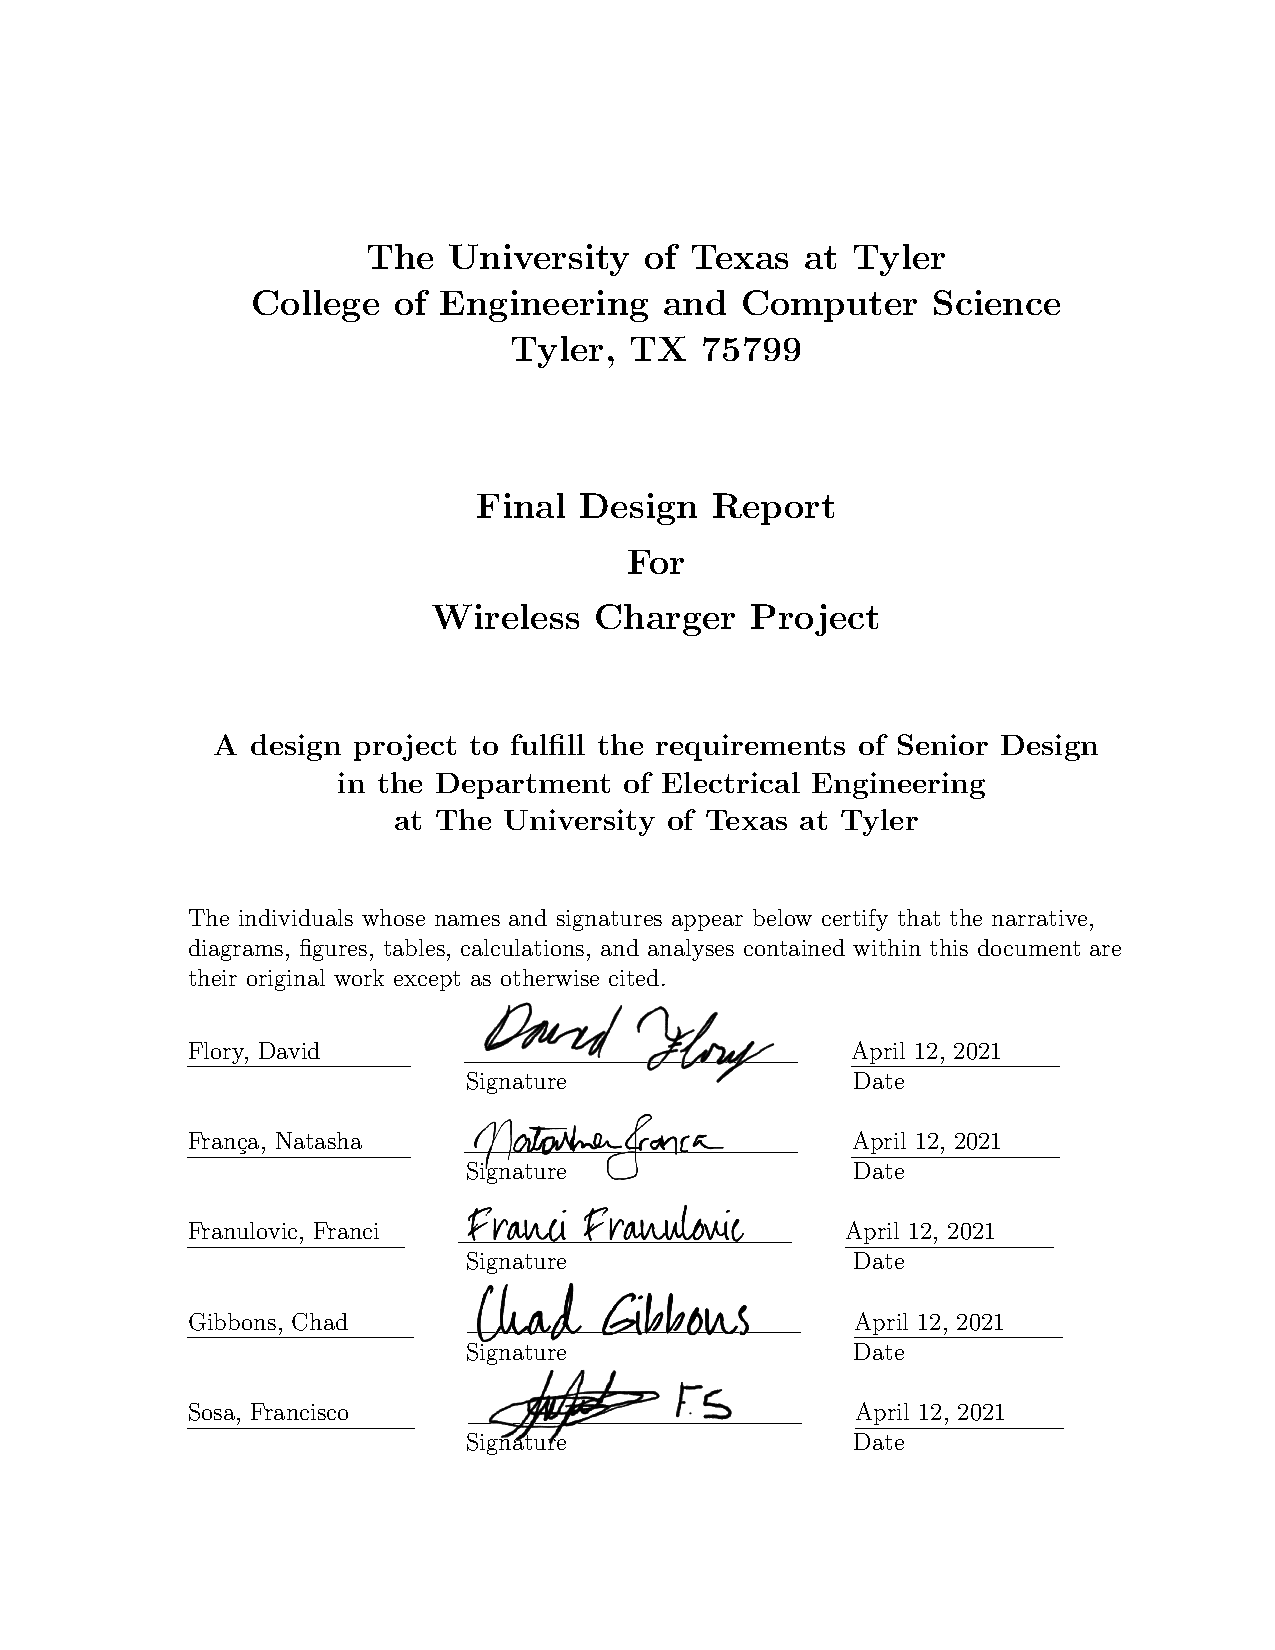
\includepdf[pages=-,pagecommand={}]{./front_page/FDR_front_page_signed.pdf}

\pagenumbering{gobble}

\pagebreak

\section*{Executive Summary}
\pagenumbering{roman}
\indent \indent
The team proposes to design and prototype a managed, 30 watt wireless resonant charger for use with lithium-ion battery packs. It will be a versatile solution to the problem of powering autonomous mobile devices fitted with moderately sized battery packs of approximately four to six 18650 cells configured for 7.4 to 14.7 volts nominal output. With a preliminary cost estimate of \$300, it fills a gap between inexpensive inductive chargers in the 5 watt range and custom 90 watt robotic power systems with an entry level price of \$2000.\\ \indent

Our charging system will be made of two essential components: a transmitter and receiver. The transmitter will be supplied by standard line voltage and will be responsible for safely delivering up to 30 watts of resonant power to the receiver when in range and appropriately positioned. It will communicate status with the receiver over a Bluetooth link and will enable or disable power transmission when requested.\\ \indent

The receiver will communicate with the transmitter and to a user GUI over Bluetooth links, and optionally with the user’s own application (i.e. a robot microcontroller) over a serial link. It will be capable of delivering requested power transmission and charging status information and beginning or ending the charging process. It will disable charging on receipt of an error status from the charging circuit and will notify the user to take corrective action. Under normal conditions it will deliver power to the charging control IC, which in turn will charge the attached battery pack.\\ \indent

The charger may be configured to charge 7.4 to 14.7 nominal Li-Ion battery cells, which must have internal protection circuitry in accordance with UL1642 and IEC61960. Optimal configurations would include a 7.4V pack rated for 3.2A charging, a 11.1V pack rated for 2.2A charging, or a 14.8V pack rated for 1.7A charging.\\ \indent

To best demonstrate the full potential of our project, the team has specified optional deliverables that will be completed if time permits once the core project is completed. These stretch goals include a mobile robot capable of charging itself for continuous wireless operation and integration with a smart Li-ion battery for detailed fuel gauge and battery health status.\\

\pagebreak

\tableofcontents

\pagebreak

\listoffigures

\pagebreak

\listoftables

\pagebreak



	%%%%%%%%%%%%%%%%%%%%%%%%%%%%%%%%%%%%%%%%%%
	%														 %
	%														 %
	%		\hfill fills in the remaining spaces of the given line with spaces			 %
	%														 %
	%					\\ ends line           							 %
	%														 %
	%	Determine the number of "\hfill \\ " iterations in accord with the number of lines		 %
	%				   within you abstract.							 %
	%														 %
	%														 %
	%%%%%%%%%%%%%%%%%%%%%%%%%%%%%%%%%%%%%%%%%%




	%%%%%%%%%%%%%%%%%%%%%%%%%%%%%%%%%%%%%%%%%%
	%														 %
	%														 %
	%		The primary purpose of an abstract is to give sufficient information		 %
	%					on your report to inform 						 %
	%		researchers, students, grant providers, corporate executives, professors,  	 %
	%				professionals, or the audience of your intention			 %
	%		whether or not either reading or purchasing your report is necessary.		 %
	%														 %
	%														 %
	%%%%%%%%%%%%%%%%%%%%%%%%%%%%%%%%%%%%%%%%%%


\pagenumbering{arabic}

\section{Project Description}
\indent \indent
Our project is to design and prototype a 30 watts nominal resonant wireless charger for use with 4 to 6 cell lithium ion battery packs. It will be microcontroller managed and may be monitored and controlled by a user GUI or directly by the target application. Unlike existing customized and proprietary robotic charging systems, our product will charge a standard battery type and be suitable for both stand-alone operation and integration into the user's own design.\\ \indent

The team has been unable to discover any equivalent to our intended product for retail. The closest comparable product is a 90 watt magnetic resonance device that is marketed to businesses designing commercial drones and robotic systems. On the lower end, nearly all unbranded, low-cost wireless chargers that are available from mass online retailers supply no more than 5W via inductive charging. For a single industrial unit, the team has received a price quote for approximately \$2000 USD. Individuals and small R\&D teams that search for suitable devices through online retailers will find that these low-end transmitters are not modular and are limited to one specific purpose such as charging cell phones or key-fobs.\\ \indent

Our charging system shall employ magnetic resonance coupling to charge a lithium ion battery pack, delivering between 15 and 30 watts of power. The power transmitter and receiver will communicate as a unified system which shall provide battery management, protect against overcharging, and provide both diagnostic and telemetric information to the user and to an optional serial connection with the powered application’s control circuitry. The charging system may be monitored and controlled by the user either through an attached LCD interface or a GUI from either a Bluetooth connected PC or smartphone.\\ \indent

As an alternative to wireless charging, our intended market of hobbyists and prototype designers might consider a self-docking direct electrical connection. This is the charging method used by the Roomba, which engages with a custom dock and charges using metal contacts. While this is a cost-effective solution for a mass-produced product, wireless charging is a superior choice for autonomous mobile devices that might have a wide variety of sizes and shapes. The benefits offered by wireless charging include flexible placement of the charger, a compact charging area, greater tolerance for imperfect alignment between the charger and the target device, and the absence of exposed electrical connections.\\ \indent

To best demonstrate the full potential of our project, the team has specified optional deliverables that will be specified in detail once the core project is completed and tested. They include a mobile robot capable of charging itself for continuous wireless operation, fully integrated with a smart Li-ion battery for detailed fuel gauge and battery health status.\\ \indent

The team holds that a moderate power, low cost wireless charger with accessible telemetry will be useful to a small but important market of robotics hobbyists and developers, who at present are not being served by either proprietary business-to-business solutions or the low power, poorly documented inductive chargers available on the hobby market.\\
\hfill 
\begin{figure}[h!]
\centering
\includegraphics[width=0.84\linewidth]{black_box_power}
\caption{Operation Story Block Diagram}
\end{figure}
\hfill \\
\pagebreak
\section{Target Specifications and Ethical Considerations}


\begin{multicols}{2}

	% Wrap Table Example

%\begin{wraptable}[1]{2}[3]{4}
%...
%\end{wraptable}
%Number of lines (optional)
%“r” for right and “l” for left figure placement.
%Overhang (optional)
%Width to be reserved.


%\newcolumntype{C}{>{\centering\arraybackslash} m{6cm} }  %# New column type
%\newcolumntype{R}{>{\raggedleft \arraybackslash} m{6cm} }  %# New column type

\begin{wraptable}{l}{0.95\linewidth}
\centering
\caption{Receiver Specifications}
\begin{tabular} {| r | c | }
\hline
\parbox{0.45\linewidth}{\raggedleft \hfill \\ Charge time \\  (4Ah Battery Pack)\\} & 5 Hours Max\\
\hline
Battery pack voltage & 14.2 V  \\
\hline
\parbox{0.45\linewidth}{\raggedleft \hfill \\  Coupling Efficiency \\ Transmitter to Receiver\\[0.4em]} & 90\%\\
\hline
\parbox{0.45\linewidth}{\raggedleft \hfill \\  AC-DC \\ Conversion Efficiency} & 80\%\\
\hline
\parbox{0.45\linewidth}{\raggedleft \hfill \\  Charging Controller \\  DC-DC converter} & 85\%\\[0.4em]
\hline
\parbox{0.45\linewidth}{\raggedleft \hfill \\  Overall Receiver \\  Conversion Efficiency} & 61.2\%\\[0.4em]
\hline
\parbox{0.45\linewidth}{\raggedleft \hfill \\  Maximum Battery \\ Charging Current} &   \parbox{0.45\linewidth}{\centering 1.25 A (14.7 V \\ battery pack)}\\
\hline
\parbox{0.45\linewidth}{\raggedleft \hfill \\  Charger Subsystem \\  Charge Protocol} &  \parbox{0.45\linewidth}{\centering \hfill \\  Constant Current \\Constant Voltage \\(Li-ION Battery)}\\
\hline
Battery Type &   \parbox{0.45\linewidth}{\centering\hfill \\  Lithium-Ion \\ (4 x18650 in Series or 2P4S Configuration)}\\
\hline
\parbox{0.45\linewidth}{\raggedleft \hfill \\  Power Negotiation} &  \parbox{0.45\linewidth}{\centering\hfill \\ Bluetooth 5 LE\\}\\
\hline
\parbox{0.45\linewidth}{\raggedleft \hfill \\  Transmitter Locator \\ Method \\[0.4em]} &   \parbox{0.45\linewidth}{\centering \hfill \\  RF Localization  [Bluetooth]}\\
\hline
Deliverable Demo &   \parbox{0.45\linewidth}{\centering \hfill \\  Self-Moving Device (Robot)}\\
\hline
Telemetry &   \parbox{0.45\linewidth}{\centering \hfill \\  Report State \\to GUI Device}\\[0.4em]
\hline
LCD display &   \parbox{0.45\linewidth}{\centering \hfill \\  Diagnostic Character \\String Display}\\
\hline
\end{tabular}
\end{wraptable}
 
\vfill
\columnbreak
%%%%%%%%%%%%%%%%%%%%%%%%%%%%%

\begin{wraptable}{l}{0.95\linewidth}
\centering
\caption{Transmitter Specifications}
\begin{tabular} {| r | c | }
\hline
Operating frequency & 13.56 MHz\\
\hline
RF power output & 30 W\\
\hline
Max operating range & 30 cm\\
\hline
DC Power supply  & 12V 5A max.  \\
\hline
\parbox{0.45\linewidth}{\raggedleft  Conversion Efficiency\\ DC-AC\\[0.4em]}  & 80\%\\
\hline
Telemetry &\parbox{0.48\linewidth}{\centering Report State \\to GUI Device\\[0.4em]}\\
\hline
\end{tabular}
\end{wraptable}



\begin{wraptable}{l}{0.95\linewidth}
\centering
\caption{Communication Link Specifications}
\begin{tabular} {| r | c | }
\hline
\parbox{0.45\linewidth}{\raggedleft Communication Medium \\[0.4em]} &  \parbox{0.48\linewidth}{\centering Bluetooth 5 LE}\\
\hline
\parbox{0.45\linewidth}{\raggedleft Protocol} &  \parbox{0.48\linewidth}{\centering TBD}\\
\hline
\end{tabular}
\end{wraptable}


\begin{wraptable}{l}{0.95\linewidth}
\centering
\caption{GUI Specifications}
\begin{tabular} {| r | c | }
\hline
\parbox{0.45\linewidth}{\raggedleft GUI OS} & \parbox{0.48\linewidth}{\centering \hfill \\ WinOS, IOS, \\ Linux, \& Android}\\[0.4em]
\hline
\parbox{0.45\linewidth}{\raggedleft License} &    \parbox{0.48\linewidth}{\centering LGPL 3.0} \\
\hline
\parbox{0.45\linewidth}{\raggedleft Software Architecture} &   \parbox{0.48\linewidth}{\centering \hfill \\ Model-Controller-View (MCV) Architecture\\[0.4em]} \\
\hline
\parbox{0.45\linewidth}{\raggedleft Delivery Model} &   \parbox{0.48\linewidth}{\centering \hfill \\ Open Source \\ (Free App Download)} \\[0.4em]
\hline
%\parbox{0.45\linewidth}{\raggedleft Deployment Model} &   \parbox{0.45\linewidth}{\centering Open Source / Free To Download App} \\
%\hline
\end{tabular}
\end{wraptable}
 \hfill \\
 \vfill 

\end{multicols}

%%% Subsystem dependencies should be STRICTLY about dependency inversion.   REMOVE all content pertaining to communication of functionality.
\subsection{Subsystem Dependencies}
\indent \indent
There are three modular components of the wireless charger project: the transmitter, the receiver, and the GUI. Additionally, in order to demonstrate a POC, this project will include a robotic subsystem that accepts the receiver as an onboard module.  Thus, the project is concerned with four modular components that fall within a hierarchy of control.  This evaluation of how each component and their subsystems subordinate to one another is critical for firmware and software development methodologies implementation.\\ \indent

The most independent component is the robot.  This means that the robot does not ask anything from the receiver, transmitter, or GUI but must accept transmissions to it and perform the task associated with the particular communiqué and any status report is read by the other components dependent upon the robot for information.  The furthest extent of interaction on part of the robot component for the POC would be to validate a networking handshake during Bluetooth communications.\\ \indent

The next most independent component is the transmitter on account to its responsive or passive functionality.  The transmitter shall respond to the receiver's requests for charging and periodically emit RF-pings to provide the receiver with positional data.  The transmitter will not consider whether a ping is received nor search for a receiver unless instructed to do so by the user via the project's GUI.  The transmitter must have fail-safe protocols within its subsystems from its microcontroller.\\ \indent

Each receiver is independent of one another as well as from the GUI.  A receiver would be dependent upon the robot accepting its telemetry's locating feed as well as the transmitter pings and power to provide any value.  The receiver will monitor the battery status and seek to induce proper voltages and currents in order to charge the battery.  It will provide the transmitter with a distance vector to validate that it is close enough to begin charging via magnetic coupling.  Furthermore, it will inform the transmitter to shut off by ceasing network authentication after detecting that the battery is charged or any system error is detected. The receiver shall be pairable to a specific transmitter before it is installed into a robot in order to maintain full operability in the absence of a user running The Project's GUI Application.\\  \indent

The completely dependent component is the GUI, i.e. the Graphical User Interface.  For the purposes of this section, the GUI will be considered indistinguishable from the Project's Application that runs the GUI and fulfills all its functionality.  It will have the adaptability to communicate with the receiver's enclosing robot.  The GUI primarily fulfills the need to monitor the status of the transmitter and receiver in real time.  It can be used to monitor the battery's charge or to turn off either the receiver or the transmitter directly as a bypass.  The GUI will be compiled on any OS that Qt5 supports and downloadable for free off the internet.  The GUI will add value to the Wireless Charging System as a whole without being a critical component.

\subsection{Hardware Components}
\begin{figure}[h!]
\includegraphics[width=0.92\linewidth]{power_supply_diagram}
\caption{Power Supply of Transmitter and Receiver Subsystems}
\end{figure}
\indent
There are two hardware components to the system: a transmitter and receiver.  Additionally, a third hardware component shall be included for the scope of this system's proof of concept (POC), i.e. a robot with the wireless charger receiver module on-board.  The POC demonstration will exhibit the charging of onboard batteries, locating the robot via the receiver's telemetry, an error test with only the receiver's attached LCD Status Display, and provide real-time feedback on a GUI via Bluetooth communication.  The onboard battery pack is to provide power to both the robot and the receiver power when uncoupled from the transmitter. 
\begin{figure}[h!]
\centering
\includegraphics[width=0.41\linewidth]{transmitter_diagram.png}
\includegraphics[width=0.532\linewidth]{receiver_diagram.png}
\caption{Transmitter and Receiver Block Diagrams}
\end{figure}
\hfill \\

\subsubsection{Transmitter:} 
The transmitter provides power wirelessly and communicates asynchronously with the receiver.  The receiver converts that power to proper voltage levels for battery charging.  Telemetry and robot subsystems shall operate on the battery's power.  Both the transmitter and receiver will negotiate power transmission and the wattage thereof.  The transmitter will not be on at all times.  The transmitter will start providing RF power only while the receiver requests power.  Also, power delivery will be disabled if the coupling efficiency drops below 90\%.  Upon undesired decoupling, the receiver will provide its robot correctional vectors that can be used to reposition the robot for optimal charging. This receiver's positional correction will give an added benefit of preventing bystanders from exposure to strong electromagnetic fields. \\ \indent

Both of the system's hardware components will require firmware for their microcontrollers to fulfill their targeted deliverables.  This firmware is specific to their design and must be developed as part of the project.  Their firmware must permit communication with external devices running the project's graphical user interface (GUI) over Bluetooth.\\

The transmitter takes power from a DC source and generates an electromagnetic field using an RF amplifier and antenna. For safety and efficiency concerns a power negotiation protocol between the transmitter and the receiver is required for safe and efficient operation. The transmitter will display important parameters on the LCD display mounted on its enclosure and more detailed data will be transmitted to the remote PC, tablet or phone via wireless link.\\

\noindent
$\cdot$ External power supply  12V, 5A (off the shelf power supply) will be used to provide power to the system.\\
$\cdot$ Internal DC-DC converter will be used to step down input voltage to appropriate levels for internal devices. (The transmitter will require at three different voltage levels for powering  microcontroller, Bluetooth, LCD, RF generation stage and RF amplifier.)  \\
$\cdot$ DC to RF converter consists of an RF oscillator followed by a buffer stage.\\% The buffer stage must be capable of driving GAN FET in the output stage.\\
$\cdot$ Buffered RF signal  is supplied  to the class E amplifier that drives the tuned transmitter LC circuit.\\ % For the best possible efficiency an GAN FET will be used to drive transmitter coil \\
$\cdot$ Microcontroller is used to control the transmitter (power negotiation and safety), data collection and communication coordination.\\ %The MSP 430 microcontroller series  has all standard peripherals (SPI, I2C, UART) and 12-bit ADC that can be used for sampling voltages and currents. This type of microcontroller is planned to be used in the receiver subsystem. Therefore, it makes sense to use the same processor in the transmitter part since this part is sufficient for this design requirement. Using the same microcontroller in both parts will reduce cost and development time.\\
$\cdot$ The LCD is used to display selected parameters such as RF amplifier supply current, input power current and coil RF voltage.  This display will be a simple two row charter display. \\
\hfill \\
$\cdot$ The Bluetooth module will be used as a communication device for telemetry and power negotiation between the power transmitter and receiver.\\
$\cdot$ Entire transmitter  will be designed and assembled on a single PCB.%\\

%Goal remove bullet points. Justification : takes up too much space for too little benefit.

\subsubsection{Receiver:} 
%%% David wrote content in PDD missing from here
The receiver is responsible for battery management, conversion of RF to DC power for charging, and for communicating status with the transmitter, the device under power, and the user via a local LCD interface or remote GUI. Battery management functions will include the monitoring of charge level, battery temperature, and charging current and voltage. The receiver will detect a low battery condition, provide telemetry to the powered device, and will request RF power transmission from the transmitter when in charging range. A single microcontroller will manage all receiver functions with support from appropriate battery management and wireless communication modules.

%$\cdot$ The receiver consists of a tuned LC circuit  followed by RF to DC converter. %The  RF to DC converter will be a schottky diodes rectifier bridge. It is critical that this part uses high speed switching diodes for efficient RF to DC conversion.  Received DC power is regulated using a switching DC-DC converter in order to provide appropriate voltage levels for battery charger circuits. \\
%$\cdot$ The Battery charger circuit  has charger controller and battery management for constant battery monitoring (charge/discharge current, capacity and temperature).\\ %This part will be developed using available integrated circuits from Texas Instruments (TI). The Buck-boost converter should be considered for the  battery charger implementation. There are many available choices available for lithium ion battery charger controllers. One good choice for this application is BQ25790.  This integrated circuit  is controlled using the I2C interface. It can charge up to four battery cells with currents up to  5 A. The charger  operates as a buck-boost converter which allows wide input operating voltage. This IC can be configured to charge up to 4 batteries.\\
%$\cdot$ Battery management functionality will be implemented using a dedicated integrated circuit.\\ %One good choice to realize battery management  with protection is  BQ3055CEDV. This is a low power integrated circuit that provides temperature measurement cell balancing, voltage measurement and current measurement. This IC also has a gas gauging function (it provides information about current state of  battery capacity).\\
%$\cdot$ Microcontroller is used for data collection, power negotiation, communication management and robot controller. The microcontroller must be low power in order to make the battery charger efficient.\\ %One good choice for this application is the MSP430 series. The MSP 430 microcontroller series  has all standard peripherals (SPI, I2C, UART) and 12-bit ADC that can be used for sampling voltages and currents.\\
%$\cdot$ The LCD is used to display selected parameters such as battery voltage, current and remaining battery charge capacity.\\ %% c.f. David on PDD

\subsubsection{Robot:}
As a proof of concept for the wireless charger we will integrate it into an example robotics application. Our mobile robotics application will interpret charger telemetry to recognize a low battery condition and position itself appropriately for charging. \\
$\cdot$ Custom PCB will be required for the microcontroller and stepper motor drivers. Electronic circuit for this part will be independent from the charger circuit.

%Goal remove bullet points. Justification : takes up too much space for too little benefit.

\subsubsection{Software:}
The inter-platform software will provide the user an interactive suite of realtime information via a graphical user interface (GUI).  The GUI shall be modular and have the ability to incorporate further functionality, be it communicating with the robot or implementing automated communications to the hardware components.\\
%%% MERGE %%% The Transmitter, Receiver, and remote GUI will all require custom software components. The Transmitter and Receiver will have custom microcontroller firmware appropriate to their functions. The GUI will be based on an appropriate portable programming framework, and will be intended to give the user easy access to battery management data and charging status
%%% MEREGE into content %%% $\cdot$ Telemetric data transmitted using Bluetooth will be displayed in GUI.\\

%Goal remove bullet points. Justification : takes up too much space for too little benefit.

\hfill \\
\pagebreak
\hfill \\


\begin{figure}[h!]
\includegraphics[width=0.9\linewidth]{total_diagram}
\caption{Subsystem Relational Block Diagram}
\end{figure}

\pagebreak

 
\subsection{Ethical and Professional Considerations}

\subsubsection{Public Health:}
Life preserving medical equipment requires concern in the transmission of powerful RF charging signals that may interfere with the medical equipment. We will adhere to FCC standards for intentional radiators and ensure that the charger transmitter does not exceed FDA guidelines for RF emission. Our design will be informed by the guidelines of the National Council on Radiation Protection and Measurements (NCRP) and the Institute of Electrical and Electronics Engineers (IEEE).
%This device provides a means of attention to the expulsion of battery acid or other wastes from the battery chamber.  It seeks to minimize harmful by-products in the use of batteries by properly maintaining stable temperatures and observing relationships within the battery chamber itself via a thermal sensor.\\ \indent
 
\subsubsection{Safety and Welfare:}
Our design may contribute to public safety and welfare by easing the development of robotic systems intended to handle hazardous materials, work in narrow spaces, high temperature environments, or in vacuum. We will follow industry best practices for safe charging, such as current limiting and temperature monitoring, to minimize the risk of battery failure.

\subsubsection{Global Factors:}
The pressures of governing bodies are to be taken into consideration in any choice this project takes; however, we are primarily concerned with the US governing bodies and then the EU bodies in order to streamline our development process to hit the largest market base possible.  Additionally, Canadian and Mexican regulations would be considered as immediate market options.\\
In an alternate vein, there are sourcing questions that must be investigated before production in order to conform with internation laws and prevent being banned from specific global markets whether at home or abroad.

\subsubsection{Societal factors}
The source code will be educational as well as providing value to the device itself.  The design's modular intention will permit versatile implementations at work or at home.  The product should serve influenceable groups such as teenagers, helping them enter STEM related fields.\\
The product as a whole should be considered in a way that would encourage further education in the classroom in physics.  Likewise, the production of the product should foster a community between the product's programmers and engineers.

\subsubsection{Environmental factors:}
This concern requires continual attention for any anomalies concerning the battery cells.  The device cannot account for all of these concerns, but should maintain labeling that makes the customer aware of such concerns that may be caused by their device.  The project must provide a means of emergency shut off by some interrupt port that is always active.  The operating robot, the user via a GUI, and the receiver itself must have this ability to turn off the charging feature of the receiver.

\subsubsection{Economic factors:}
The device could fulfill legal requirements for a client, and, in that case, a custom suite would be developed in the software at a premium to satisfy a client's needs.  Additionally, creating a lightweight, low-cost production process is critical in maximizing profits.  The open-source market also provides extensive free advertising momentum when capitalized successfully.  Additionally, the product would assist in producing other products, especially in research and development. \\
% Special considerations will have to be made to including an ``In-App Purchases'' model, namely customer security and privacy concerns.  
\begin{table}[h!]
\centering
\caption{Ethical and Professional Considerations}
\begin{tabular} {| r | c | }
\hline
\parbox{0.3\linewidth}{\raggedleft Public Health} &   \parbox{0.65\linewidth}{\hfill \\
$\cdot$ Medical Equipment RF Exposure \\ $\cdot$ Electrical Shock \\ $\cdot$ Chemical Exposure}\\
\hline
\parbox{0.3\linewidth}{\raggedleft Safety and Wellness} &   \parbox{0.65\linewidth}{\hfill \\
$\cdot$ RF Bandwidth Jamming \\ $\cdot$ Electrical Shock \\ $\cdot$ Chemical Exposure}\\
\hline
\parbox{0.3\linewidth}{\raggedleft Global Factors} &   \parbox{0.65\linewidth}{\hfill \\
$\cdot$ International Governing Bodies \\ $\cdot$ Sourcing Restrictions \\ $\cdot$ Inter-Market Penetrability}\\
\hline
\parbox{0.3\linewidth}{\raggedleft Societal Factors} &   \parbox{0.65\linewidth}{\hfill \\
$\cdot$ Open-Source Capitalization\\ $\cdot$ STEM Educational Resources \\ $\cdot$ Professional Organizations \\ $\cdot$ Customer Privacy \& Security}\\
\hline
\parbox{0.3\linewidth}{\raggedleft Environmental Factors} &   \parbox{0.65\linewidth}{\hfill \\
$\cdot$ Chemical Pollution\\ $\cdot$ User Environmental Awareness\\ $\cdot$ Emergency Shut Off Cases}\\
\hline
\parbox{0.3\linewidth}{\raggedleft Economic Factors} &   \parbox{0.65\linewidth}{\hfill \\
$\cdot$ Open-Source Capitalization\\ $\cdot$ Specialty Clientele\\ $\cdot$ Rapid Agile-Deployment\\ $\cdot$ Light-Weight Production}\\
\hline
\end{tabular}
\end{table}
\hfill \\

\section{Engineering Standards and Constraints}

\subsection{Safety Constraints Mandated by Government and Possible Risks of Wireless Power Transfer (WPT)}

\indent \indent
In the United States, two government agencies are responsible for regulations regarding RF exposure safety. Those agencies are the Federal Drug Administration (FDA) and Federal Communications Commission  (FCC). Both agencies have their own set of rules that are similar.

\hfill \\
\pagebreak


\subsubsection{FDA Safety Regulations}
There are safety concerns about exposure to strong electromagnetic fields. The FDA divides wireless chargers into two categories:\\
$\cdot$ \indent Proximity type (where the device is in contact with the charger)\\
$\cdot$ \indent Directed (beamed) delivery across space\\

\indent
Since this design fits in the category of  proximity chargers FDA rules for this type of charger must be followed. According to FDA Resonant proximity charges have resonant LC circuit which improves range and efficiency. FDA clearly states that higher power RF transmitters pose a higher risk. Since the wireless charger is a powerful RF transmitter there are concerns about effects of the wireless charger to metal objects such as rings and implanted medical devices and other wearable metal pieces.\\

\indent
The FDA clearly states that higher power products pose a higher risk and there are concerns about effects of the wireless charger to metal objects such as rings implanted medical devices and other wearable metal pieces. Also, the FDA has concerns regarding WPT in terms of electromagnetic interference with medical devices or disruption of device communications. Therefore, engineering controls must be sensitive and reliable enough to prevent injury. Also, it is important to keep in mind that not all existing products implement electromagnetic safety. Hence, some existing products may malfunction if they are exposed to strong electromagnetic fields.  \\

\subsection{Relevant FDA Safety Regulations and Standards}
\indent \indent
FDA has multiple standards and regulations. Since our device will use an RF transmitter  for power transfer, Title 21 code CFR 1000.15(b) is applicable \cite{21cfr1000}. \\

\indent
IEEE C95.1-2005 standard defines guidelines regarding RF power density for localized and whole-body exposure to electromagnetic fields generated by the RF emitter \cite{ieeec95} (in our case transmitter). Those two standards address exposure to electromagnetic fields. In order to address this rule, we are limiting our transmitter power to 30W\cite{ieeec95}. A power negotiation protocol will be used to enable the charger transmitter only when the receiver is present and properly placed in the front of the charger. \\

\indent
Exposure limits are clarified in IEEE Standards Interpretations for IEEE Std C95.1-2005. IEEE Standard for Safety Levels concerning Human Exposure to Radio Frequency Electromagnetic Fields, 3 kHz to 300 GHz. According to interpretation from  the IEEE  Standards Interpretations the whole body exposure is limited to 0.08W /kg and localized exposure is 2W/kg.
Since the transmitter will operate on the frequency that ranges from 100kHz to 1GHz exposure levels in this rule is applicable  to our design.\\
\hfill \\
\pagebreak
\hfill \\
\indent
The FCC also addresses concerns about  RF exposure considerations for low power consumer wireless power transfer from FCC. % Seek out FCC regulations from bookmarked webpage
WPT devices must satisfy RF exposure limits from FCC standard KDB 680106 D01 \cite{fcc15}\cite{fcc18}\cite{fccsum}. 
All wireless power transfer devices that operate above 9kHz are considered intentional radiators and they are subject to FCC rules. \\

\indent
FCC sets  regulations and norms  for WPT devices and it is mandatory to certify WPT devices prior making them available on the market. Those rules include unwanted emissions limits in order to prevent electromagnetic interference. Also, FCC sets frequency allocation plans. According to the frequency allocation plan frequency 13.56MHz is available for wireless power transfer devices in the USA. \\

\indent
 FCC has established a regulatory framework for wireless power transfer. According to the FCC information, the charging mode is certified under FCC Part 18 \cite{fcc18} and the communication part is certified under Part 15 \cite{fcc15}\cite{fccsum}. Given FCC requirements it is feasible to use an already certified module for wireless communication such as Bluetooth, Zigbee, or Wi-Fi. That way only WPT circuits would be subject to certification according to FCC Part 18 \cite{fcc18}. When all available regulations are considered the best operating frequency for the wireless charger is most likely 13.56MHz since that frequency may become the worldwide standard for WPT. Also, this frequency will allow WPT transfer using magnetic resonance which does not require very precise positioning and matching charger transmitter coil. The power limit ( max. 30W) will be more than enough for this application. \\

\indent
Given FCC requirements, it is feasible to use an already certified module for wireless communication such as Bluetooth. Bluetooth is covered by the IEEE 802.15.1 standard and is widely used in many devices and is licensed worldwide \cite{ieee802}.

\subsubsection{Safety Standards for Lithium-ion Battery Chargers}
We plan to follow the IEEE 1625-2008 Standard \cite{ieee1625} for rechargeable batteries for multicell mobile computing devices because this device is universal and can be considered as a computing device. This standard provides guidelines on implementing the safety controls for the design and manufacture of lithium-ion (Li-ion) and lithium-ion polymer (Li-ion polymer) rechargeable battery packs \cite{ieee1625}. Safety guidelines are addressing the fire hazard due to charger or battery failure \cite{ieee1625}.

\subsubsection{WPT frequency plan and power limits international overview}
According to ETSI (European Standards Organization), there are certain frequencies and prescribed maximum power levels for wireless charging. Some of those frequency bands are candidates for international harmonization (those frequency bands will be dedicated to WPT transfer). At this moment there is no agreement on which frequency band will be used for WPT worldwide.\\
\hfill \\
\pagebreak
\hfill \\
\indent
ETSI documentation  gives an overview of different frequencies for the implementation of WPT systems. According to ETSI 13.553 – 13.567 MHz band is currently used for power transfer for the following power classes P$<$1W, 1W$<$P$<$5W, 5W$<$P$<$31.5W \cite{en55011}. This is an International standard that covers European Union EU and European economic area (EEA) as well as many other regions (Parts of Africa, Asia and  Australia )  follow European Union (EU) regulations related to this matter.\\

\indent
EN 55011:2016 international standard for electromagnetic compatibility. This standard applies Industrial, scientific and medical equipment and  addresses  radio frequency disturbance. This standard sets limits to electromagnetic emissions from the product. In order to avoid creating disturbance in RF communication the wireless charger electromagnetic emissions must be below the limit prescribed in this standard. This is achieved by proper circuit design and using  low pass filters on all connections that are exposed to the user.
\hfill 
\begin{table}[h!]
\centering
\caption{Overview of Relevant Standards}
\begin{tabular} {| r | c | }
\hline
\parbox{0.17\linewidth}{\centering Organization} &   \parbox{0.772\linewidth}{\centering Engineering Standards}\\
\hline
\parbox{0.17\linewidth}{\raggedleft IEEE} &   \parbox{0.772\linewidth}{\hfill \\
IEEE C95.1-2005\\
This standard defines exposure limits to the electromagnetic field \\
This standard is adopted in many safety standards. \\
IEEE 1625-2008 \\
Standard for rechargeable batteries for multicell mobile computing devices.\\
IEEE 802.15.1 Bluetooth standard \\
}\\
\hline
\parbox{0.17\linewidth}{\raggedleft Government} &   \parbox{0.772\linewidth}{\hfill \\
FCC Part 15, FCC part 18\\
RF Power levels and communication links are defined by FCC Part 15 and Part 18.\\
The RF transmitter power level limits in the US are much higher than in some other countries.\\
FDA: 21 CFR 1000.15 FCC: KDB 680106 D01   \\
Both standards define exposure limits to electromagnetic fields.\\
The limits will be satisfied if the transmitter power is limited to 5W.\\
Higher power levels are allowed if proper safety measures are implemented.\\
}\\
\hline
\parbox{0.17\linewidth}{\raggedleft International} &   \parbox{0.772\linewidth}{\hfill \\
EN 55011:2016\\
This standard defines limits for unwanted emissions in the RF spectrum above 30MHz. \\
The proposed WPT charger system must follow limitations for unwanted emissions.\\
}\\
\hline
\end{tabular}
\end{table}
\hfill \\
\pagebreak
\hfill
\begin{table}[h!]
\centering
\caption{Overview of Constraints}
\begin{tabular} {| r | c | }
\hline
 &   \parbox{0.772\linewidth}{\centering Technical Description}\\
\hline
\parbox{0.21\linewidth}{\raggedleft Cost} &   \parbox{0.772\linewidth}{\hfill \\
\$320 Estimated Prototype Cost
%Breakdown:\\
%\$120 Receiver\\
%\$70 Transmitter\\
%\$130 Robot\\
}\\
\hline
\parbox{0.21\linewidth}{\raggedleft FDA} &   \parbox{0.772\linewidth}{\hfill \\
FDA: 21 CFR 1000.15 FCC: KDB 680106 D01   \\
Both standards define exposure limits to electromagnetic fields.\\
The limits will be satisfied if the transmitter power is limited to 5W.\\
Higher power levels are allowed with proper safety measures.
}\\
\hline
\parbox{0.21\linewidth}{\raggedleft Government} &   \parbox{0.772\linewidth}{\hfill \\
FCC Part 15, FCC part 18\\
RF Power levels and communication links sic FCC Part 15 and Part 18.\\
The RF transmitter power level limits in the US are much higher than other countries. EU rules power requirements satisfy US regulations.
}\\
\hline
\parbox{0.21\linewidth}{\raggedleft International} &   \parbox{0.772\linewidth}{\hfill \\
EN 55011:2016\\
This standard defines limits for unwanted emissions in the RF spectrum above 30MHz. \\
The proposed WPT charger system must follow limitations for unwanted emissions.
}\\
\hline
\parbox{0.21\linewidth}{\raggedleft Speed} &   \parbox{0.772\linewidth}{\hfill \\
 Recharge speed 5 hours (for 5. Ah battery pack 14.4V)
}\\
\hline
\parbox{0.21\linewidth}{\raggedleft Reliability} &   \parbox{0.772\linewidth}{\hfill \\
 The charger will be able to detect improper positioning and it will monitor for power coupling efficiency. \\
 If is coupling inefficient it will provide warning and it will not start charging process. \\
The device will continuously monitor battery conditions such as charge or discharge current, voltage and temperature in order to prevent battery capacity degradation 
Power\\
RF transmitter power $<$30W  \\
Overall power supply input requirement will be $<$50W.
}\\
\hline
\parbox{0.21\linewidth}{\raggedleft Complexity} &   \parbox{0.772\linewidth}{\hfill \\
The system has two hardware parts power transmitter and the  robot with integrated power receiver with the charger battery management and battery pack 
}\\
\hline
\parbox{0.21\linewidth}{\raggedleft Manufacturability} &   \parbox{0.772\linewidth}{\hfill \\
The device design will be based on standard electronic/electrical and mechanical components that are readily available.\\
Electronic circuit assembly sic custom printed circuit board design. Two PCBs one for receiver and the other for the receiver/robot.\\
All electrical components such as batteries and motors will be standard, readily available components.\\
The design will utilize mechanical parts such as gears, shafts, and fasteners that are commonly used and readily available.
}\\
\hline
\parbox{0.21\linewidth}{\raggedleft Sustainability} &   \parbox{0.772\linewidth}{\hfill \\
This device is designed to cause minimal wear and tear to itself and any device connected to its system.  The receiver would extend the lifetime of others’ devices by providing a low-cost recharging option.
}\\
\hline
\end{tabular}
\end{table}
\hfill 
\pagebreak
\hfill \\

\section{Evaluation of Design Alternatives }	%%%% NOTE:  CHANGE ORDERING OF DOCUMENT SUBSECTIONS %%%%

\subsection{Primary Power Stage}
\indent \indent
The wireless charger and receiver system will depend on AC line power provided to the wireless transmitter unit.\\

\noindent
Options:\\
\hfill \\
\noindent
1) Direct AC connection
\begin{addmargin}[0.50cm]{0.75cm}
a)  Immediately rejected due to safety concerns and unneeded complexity.
\end{addmargin}
2) Approved 110-220 VAC to 12 VDC commercial switch-mode power supply.
\begin{addmargin}[0.50cm]{0.75cm}
a)  Advantages
\begin{addmargin}[0.50cm]{0.75cm}
i) \space\space  low cost\\
ii) \space  standard voltage\\
iii)  ready availability.
\end{addmargin}
b)  Disadvantages
\begin{addmargin}[0.50cm]{0.50cm}
i)  Additional boost stage required to provide the higher voltages required by the resonant transmitter, adding complexity and power loss.\\
ii)  Five amp input current would create undesired power losses.
\end{addmargin}
\end{addmargin}
3) Approved 110-220 VAC to 48 VDC commercial switch-mode power supply.
\begin{addmargin}[0.50cm]{0.75cm}
a)  Advantages
\begin{addmargin}[0.50cm]{0.75cm}
i) \space\space Good availability through engineering supply channels.\\
ii) \space   Relatively low input current reduces heat loss\\
iii)   Voltage near or only slightly above what is needed by the transmission stage.\\
iv)  Example: TDK-Lambda DT62PW480D
\begin{addmargin}[0.50cm]{0.75cm}
1) 48 VDC, 1.36 A maximum (65 watts)\\
2) Higher wattages and alternate manufacturers available\\
3) Note that optimal efficiency is usually obtained below maximum power draw.\\
\end{addmargin}
\end{addmargin}
\end{addmargin}


\indent
The 48 VDC primary supply was provisionally approved. It will require a step down stage to provide 5V and 3.3V logic supplies for the wireless transmitter microcontroller, class E amplifier, and support circuitry.\\

\indent
The step down buck down DC converters could either be accomplished via individual custom op amp voltage regulators or integrated buck down circuits.  Furthermore, the 5 V and 3.33 V buck down DC converters could potentially be merged into a single topology.  Custom op amp voltage regulators would take up a larger surface area as well as require excessive soldering and are thus not desirable.  The only limitation in merging the 5 V and 3.33 V buck downs into a unified topology is that the 5 V buck down would require more current to feed both outputs.  The benefit would be the reduction of parts and surface area required for the total circuit.\\

\subsection{Battery Management, Power Supply, and Target Power Delivery}
\indent \indent
Our project will convert electricity from the wireless power receiver into a form suitable for charging a cell battery. It must do so while powering its own circuitry, and it must deliver power from the batteries to the target application. Our project must also be capable of monitoring the charging process and battery charge status for both safety and diagnostic purposes. It must be able to respond to instructions and queries received from the wireless power receiver microcontroller.\\

\indent
When implementing a rechargeable battery management system, it is first necessary to decide what battery chemistries the system will support. The team considered NiMH and Li-ion chemistries and favored the latter due to the far greater power density. The team had already selected a mobile robot as an ideal example application for our charger. It was clear that the performance and user appeal of our wireless charger would be much greater if it could utilize the higher-performance battery chemistry. The team understood that there would need to take special care that our charge circuitry would manage these high performance batteries safely.\\
\hfill \\
The following requirements were identified for the battery management system:\\
\hfill \\
1.) DC to DC conversion from the wireless power receiver to a form appropriate for \\ \indent the charging and power supply circuits.\\
2.) Charging appropriate for battery chemistry, i.e. constant current stage followed by a \\ \indent constant voltage stage.\\
3.) Temperature monitoring and protection against overcharging.\\
4.) The ability to vary charging currents in response to varying levels of wireless power, \\ \indent either automatically or in response to commands from the wireless receiver control \\ \indent unit.\\
5.) The ability to draw operating power from batteries and charger while charging is in \\ \indent progress (i.e. PowerPath).\\
6.) The ability to detect a low battery condition, which may or may not include more \\ \indent detailed fuel gauge capabilities.\\
7.) The ability to control charging behavior as needed in response to demands from the \\ \indent wireless power receiver microprocessor or user controls.\\
8.) The ability to report telemetry to the wireless power receiver microprocessor or user.\\
\hfill \\
\pagebreak
\hfill \\

\indent
There are many available integrated solutions that could meet the above requirements. In order to narrow down the possibilities the following choices must be made:\\

\noindent
1) Battery chemistry
\begin{addmargin}[0.50cm]{0.75cm}
a) Lithium-Ion\\[0.25em]
b) NiMH option\\
c) Multi-chemistry: rejected due to limited hardware options, complexity, and \\ \indent safety concerns.
\end{addmargin}
2) Linear vs. Switching input stage and input voltage range
\begin{addmargin}[0.50cm]{0.75cm}
a) Linear
\begin{addmargin}[0.50cm]{0.75cm}
i) Usually seen on small, single or dual cell chargers.
\end{addmargin}
b) If Switching:
\begin{addmargin}[0.50cm]{0.75cm}
i) Buck: may make an additional DC/DC stage unnecessary.\\
ii) Boost: not likely to be necessary\\
iii) Buck-boost: may make an additional DC/DC stage unnecessary
\end{addmargin}
\end{addmargin}
3) Stand-alone vs. programmable
\begin{addmargin}[0.50cm]{0.75cm}
a) Jumper/hardware settings
\begin{addmargin}[0.50cm]{0.75cm}
i) Limited configuration options.\\
ii) Limited data available via status lines (i.e. over-temp condition)\\
iii) Simple implementation.
\end{addmargin}
b) I2C programmability
\begin{addmargin}[0.50cm]{0.75cm}
i) Most configuration and control issues may be worked out in software.\\
ii) Configuration may be altered during operation by firmware or \\ \indent user instructions.\\
iii) Status registers may be queried by the microcontroller at any time.
\end{addmargin}
c) SMBus programmability
\begin{addmargin}[0.50cm]{0.75cm}
i) Generally equivalent to I2C\\
ii) Libraries available for MSP430\\
iii) Automatic timeout supported
\end{addmargin}
\end{addmargin}
4) Maximum power point tracking
\begin{addmargin}[0.50cm]{0.75cm}
a) Offered as an integrated option within Analog Devices LTC4162 family.
\begin{addmargin}[0.50cm]{0.75cm}
i) May be useful depending on wireless power receiver design choices.\\
\end{addmargin}
\end{addmargin}


\noindent
Preliminary recommendations:
A fully programmable multi-cell charge controller from a modern, well-supported product line is the most flexible option. Such a device would allow many design choices to be made in software and changed if necessary.\\
\hfill \\
\pagebreak
\hfill \\
Candidates include:\\

\noindent
1) Texas Instruments: BQ257xx
\begin{addmargin}[0.50cm]{0.75cm}
a) Buck-boost power input\\
b) Supports 1-4 Li-ion cells\\
c) Options include I2C/SMBus, USB-PD, CPU throttling signals\\
d) Demo available: BQ2571x
\end{addmargin}
2) Analog Devices: LTC4162
\begin{addmargin}[0.50cm]{0.75cm}
a) Buck power input\\
b) Supports 1-8 Li-ion cells\\
c) Integrated MPPT option\\
d) Demo available: DC2038A
\end{addmargin}
3) Texas Instruments: BQ2002
\begin{addmargin}[0.50cm]{0.75cm}
a) Linear power regulation\\
b) Supports 1-4 NiMH cells\\
c) Thermistor monitoring\\
d) Standalone RC-Settable\\
\end{addmargin}

\begin{table}[h!]
\centering
\caption{Battery Charger Alternatives Evaluation Table}
\begin{tabular}{| l | l | l | l |}
\hline
\parbox{0.17\linewidth}{\centering Evaluation Basis} & \parbox{0.240\linewidth}{\centering \hfill\\ Texas Instruments BQ25790\\
} & \parbox{0.240\linewidth}{\centering\hfill\\ Analog Devices LTC4162\\} & \parbox{0.240\linewidth}{\centering\hfill\\ Texas Instruments BQ2002\\}\\
\hline
\parbox{0.17\linewidth}{\raggedleft Environmental Factors} &
\parbox{0.240\linewidth}{\hfill \\
RoHS compliant.\\
Environmental concerns with Li-ion cell production and disposal.
\\} & 
\parbox{0.240\linewidth}{\hfill \\
RoHS compliant.\\
Environmental concerns with Li-ion cell production and disposal.
\\} & \parbox{0.240\linewidth}{\hfill \\
RoHS compliant.\\
Environmental concerns with Li-ion cell production and disposal.
\\}\\ \hline
\parbox{0.17\linewidth}{\raggedleft\hfill\\ Economic Factors\\[0.5em]} &
\$2.29 per unit &
\$2.95 per unit &
\$0.786 per unit \\
\hline
\parbox{0.17\linewidth}{\raggedleft Public Health} & 
\parbox{0.240\linewidth}{\hfill \\
RoHS
\\} & 
\parbox{0.240\linewidth}{\hfill \\
RoHS
\\} & \parbox{0.240\linewidth}{\hfill \\
RoHS
\\}\\ \hline
\parbox{0.17\linewidth}{\raggedleft Social Factors} & 
\parbox{0.240\linewidth}{\hfill \\
Fully programmable charge voltage and cell configuration.\\
High power density for a wide variety of applications.
\\} & 
\parbox{0.240\linewidth}{\hfill \\
Fully programmable charge voltage and cell configuration.\\
High power density for a wide variety of applications.
\\} & \parbox{0.240\linewidth}{\hfill \\
Very simple implementation.\\
Much lower power density may limit applications.
\\}\\ \hline
\parbox{0.17\linewidth}{\raggedleft Safety and Welfare} & 
\parbox{0.240\linewidth}{\hfill \\
Full battery telemetry and temperature monitoring.
\\} & 
\parbox{0.240\linewidth}{\hfill \\
Full battery telemetry and temperature monitoring.
\\} & \parbox{0.240\linewidth}{\hfill \\
Thermistor monitoring. \\
Fewer safety concerns with NiMH chemistry. 
\\}\\ \hline
\parbox{0.17\linewidth}{\raggedleft Global Factors} & 
\parbox{0.240\linewidth}{\hfill \\
None identified; may be used worldwide.
\\} & 
\parbox{0.240\linewidth}{\hfill \\
None identified; may be used worldwide.
\\} & \parbox{0.240\linewidth}{\hfill \\
NiMH cells may be more readily available in some markets.
\\}\\ \hline
\parbox{0.17\linewidth}{\raggedleft Cultural Factors} & 
\parbox{0.240\linewidth}{\hfill \\
Flexible battery configuration. 
\\} & 
\parbox{0.240\linewidth}{\hfill \\
Flexible battery configuration. 
\\} & \parbox{0.240\linewidth}{\hfill \\
Fixed battery configuration using batteries widely available by retail.
\\}\\ \hline
\end{tabular}
\end{table}
%\hfill \\
\pagebreak
\hfill \\
\indent
Our team decided to use Li-ion chemistry due to its superior performance and power density. The Analog Devices LTC4162 was chosen for its versatility, clear documentation and the availability of development hardware.

\subsection{Transmitter circuit}
\indent \indent
One very common way of driving coils at 13.56MHz is the class E amplifier. This amplifier can be realized by using discrete components available in integrated amplifiers (hybrid ICs).\\

\indent
One readily available solution for the transmitter amplifier circuit is an integrated circuit from Microsemi (part \# DRF1200).

\begin{figure}[h!]
\centering
\includegraphics[width=0.9\linewidth]{microsemi_ppg}
\caption{Microsemi Reference Design Kit for DRF1200 \cite{mdpiCoil}}
\end{figure}
\indent
This DRF1200 was tested and found to meet project specifications. The manufacturer had acceptable support and documentation. The cost of the driver was \$182.80, which would have added unacceptable costs to the design. With a maximum 1 kW output, it also far exceeded the project’s 30 W power requirement \cite{mdpiCoil}.\\

\indent
A very high voltage across the transmitter coil can be developed at high output powers in class E amplifier designs. This voltage could be as high as 1kV$_{p-p}$. This is a potential electric shock hazard. A possible safer alternative to the class E amplifier is a push-pull driver, commonly used in low-frequency WPT designs but can extend to 13.56 MHz.\\
\hfill \\
\begin{figure}[h!]
\centering
\includegraphics[width=0.9\linewidth]{circ_push_pull}
\caption{Singe-Stage and Push-Pull Topology Comparison \cite{ecceHarmonicFiltered}}
\end{figure}
\hfill \\
\indent
The push-pull topology utilizes two power transistors for driving in a way that one transistor is on and the other is off. This design would have required a complex gate driving circuit and it as well required a circuit that generates two signals, 180 degrees out of phase for the power MOSFETs gate drive. In this design, the load impedance was not required to have a tuned network on the output \cite{ecceHarmonicFiltered}.\\

\indent
Another way of driving the transmitter coil was to implement a H bridge. This design would have required two half H-bridge circuits that would have been used to drive the transmitter coils.\\
\hfill \\
\begin{figure}[h!]
\centering
\includegraphics[width=0.4\linewidth]{circ_bridge}
\caption{Half-Bridge Structure \cite{questSCI2019}}
\end{figure}\\
\hfill \\
\pagebreak
\hfill \\
\indent
This topology requires a gate driving circuit which is similar to the push-pull gate driving circuit. The load in this design was driven with full h-bridge (two half-bridge circuits). One side of the H bridge would act as a current sink while the other side would act as a current source. This approach increases the complexity and cost of the circuit beyond that of a single transistor class E amplifier \cite{questSCI2019}.\\

\indent
Powerful electromagnetic fields can cause undesired heating of nearby metal objects. Possible safety mechanisms include power negotiation and monitoring of the receiver-transmitter coupling. These safety mechanisms will prevent the transmitter from turning on without the proper receiver coupling. With effective coupling, most of the RF energy will be absorbed by the receiver and when the batteries are fully charged the receiver will then be able to send a request to the transmitter to turn off RF power.\\

\noindent
Receiver alternative designs\\

\indent
The conversion from RF power to DC is performed by the rectifying stage. The design options for this stage are relatively limited and straightforward. One common way of solving this problem is to implement a full-wave rectifier bridge implementing Schottky diodes. There are many diodes that are available for this purpose. One adequate choice was the diode part number 80SQ045N from ON Semiconductor.\\

\indent
A half-wave rectifier circuit would be the simplest and least expensive method for RF-DC conversion. This option was immediately rejected for the unacceptable loss of half the potential power of the induced AC current.\\

\indent
For safety and testing purposes, it is necessary for the receiver to be capable of determining how much power is received. The most direct approach to making this data available is to include a current sense resistor and differential amplifier to provide current sense data, and a voltage divider to provide voltage sense data. The analog output of these sensors may be measured directly by the microcontroller ADC.\\

\indent
The final design recommendation is that RF to DC conversion shall be performed by a full-wave Schottky diode rectifier bridge with sense circuits for the measurement of received power.\\

\hfill \\
\begin{figure}[h!]
\centering
\includegraphics[width=0.9\linewidth]{sim_rfdc}
\caption{Receiver RF-DC Stage}
\end{figure}\\
\hfill \\

\begin{table}[h!]
\centering
\caption{Transmitter Alternatives Evaluation Table}
\begin{tabular}{| l | l | l | l |}
\hline
\parbox{0.17\linewidth}{\centering Evaluation Basis} & \parbox{0.240\linewidth}{\centering 
Single-stage driver
} & \parbox{0.240\linewidth}{\centering 
Push-pull driver
} & \parbox{0.240\linewidth}{\centering 
H-Bridge driver
}\\
\hline
\parbox{0.17\linewidth}{\raggedleft Environmental Factors} &
\parbox{0.240\linewidth}{\hfill \\
Less efficient than push-pull or H-bridge driver
\\} & 
\parbox{0.240\linewidth}{\hfill \\
Efficient requires less energy than a single-stage driver for the same power output.
\\} & \parbox{0.240\linewidth}{\hfill \\
Efficient and complexity are similar to a push-pull solution.
\\}\\ \hline
\parbox{0.17\linewidth}{\raggedleft Public Health} & 
\parbox{0.240\linewidth}{\hfill \\
Does not have negative effects on public health if safety circuits are implemented.
\\} & 
\parbox{0.240\linewidth}{\hfill \\
Does not have negative effects on public health if safety circuits are implemented.
\\} & \parbox{0.240\linewidth}{\hfill \\
Does not have negative effects on public health if safety circuits are implemented.
\\}\\ \hline
\parbox{0.17\linewidth}{\raggedleft Economic Factors} &
\parbox{0.240\linewidth}{\hfill \\
Easy to implement. Simple driving circuit
\\} & 
\parbox{0.240\linewidth}{\hfill \\
Requires complicated driver circuit. Increases the cost of the product.
\\} & \parbox{0.240\linewidth}{\hfill \\
Requires complicated driver circuit. Increases the cost of the product.
\\}\\ \hline
\parbox{0.17\linewidth}{\raggedleft Social Factors} & 
\parbox{0.240\linewidth}{\hfill \\
N/A
\\} & 
\parbox{0.240\linewidth}{\hfill \\
N/A
\\} & \parbox{0.240\linewidth}{\hfill \\
N/A
\\}\\ \hline
\parbox{0.17\linewidth}{\raggedleft Safety and Welfare} & 
\parbox{0.240\linewidth}{\hfill \\
Requires safety circuits in order to satisfy safe RF exposure limits.
\\} & 
\parbox{0.240\linewidth}{\hfill \\
Requires safety circuits in order to satisfy safe RF exposure limits.
\\} & \parbox{0.240\linewidth}{\hfill \\
Requires safety circuits in order to satisfy safe RF exposure limits.
\\}\\ \hline
\parbox{0.17\linewidth}{\raggedleft Global Factors} & 
\parbox{0.240\linewidth}{\hfill \\
This circuit does not have any special parts. Parts are very likely available in most countries.
\\} & 
\parbox{0.240\linewidth}{\hfill \\
Special parts may be required for this design that may not be available in every country.
\\} & \parbox{0.240\linewidth}{\hfill \\
Special parts may be required for this design that may not be available in every country.
\\}\\ \hline
\parbox{0.17\linewidth}{\raggedleft Cultural Factors} & 
\parbox{0.240\linewidth}{\hfill \\
N/A
\\} & 
\parbox{0.240\linewidth}{\hfill \\
N/A
\\} & \parbox{0.240\linewidth}{\hfill \\
N/A
\\}\\ \hline
\end{tabular}
\end{table}
\hfill \\
\pagebreak
\hfill \\
\begin{table}[h!]
\centering
\caption{RF-DC Converter Alternatives Evaluation Table}
\begin{tabular}{| l | l | l |}
\hline
\parbox{0.17\linewidth}{\centering Evaluation Basis} & \parbox{0.240\linewidth}{\centering \hfill \\
Diode full-wave rectifier bridge
\\} & \parbox{0.240\linewidth}{\centering \hfill \\
Diode half-wave rectifier bridge
\\}\\
\hline
\parbox{0.17\linewidth}{\raggedleft Environmental Factors} &
\parbox{0.240\linewidth}{\hfill \\
More efficient which will reduce negative environmental effects.
\\} & \parbox{0.240\linewidth}{\hfill \\
Less efficient
\\}\\ \hline
\parbox{0.17\linewidth}{\raggedleft Public Health} & 
\parbox{0.240\linewidth}{\hfill \\
Does not have negative effects on public health.
\\} & \parbox{0.240\linewidth}{\hfill \\
Does not have negative effects on public health.
\\}\\ \hline
\parbox{0.17\linewidth}{\raggedleft Economic Factors} &
\parbox{0.240\linewidth}{\hfill \\
Simple and inexpensive design.
\\} & \parbox{0.240\linewidth}{\hfill \\
More simple and inexpensive design.
\\}\\ \hline
\parbox{0.17\linewidth}{\raggedleft Social Factors} & 
\parbox{0.240\linewidth}{\hfill \\
N/A
\\} & \parbox{0.240\linewidth}{\hfill \\
N/A
\\}\\ \hline
\parbox{0.17\linewidth}{\raggedleft Safety and Welfare} & 
\parbox{0.240\linewidth}{\hfill \\
N/A
\\} & \parbox{0.240\linewidth}{\hfill \\
N/A
\\}\\ \hline
\parbox{0.17\linewidth}{\raggedleft Global Factors} & 
\parbox{0.240\linewidth}{\hfill \\
This circuit does not have any special parts. Parts are very likely available in most countries.
\\} & \parbox{0.240\linewidth}{\hfill \\
This circuit does not have any special parts. Parts are very likely available in most countries.
\\}\\ \hline
\parbox{0.17\linewidth}{\raggedleft Cultural Factors} & 
\parbox{0.240\linewidth}{\hfill \\
N/A
\\} & \parbox{0.240\linewidth}{\hfill \\
N/A
\\}\\ \hline
\end{tabular}
\end{table}
\hfill \\
\pagebreak

\subsection{Wireless Communications}
\subsubsection{Ultra-Wideband}
This communication technique is designed for short-range transmission, and enables charging of multiple devices of high bandwidth data. Used to relay data from one device to another within a maximum distance of 30 feet. UWB waveforms are different from other carrier waves in that they are short in duration. They also offer optimal enhancements in areas including communications, radar and positioning/ranging. In communications systems, large RF bandwidths can transmit data rates of gigabits per second. UWB can be also used as communication links that involve sensors, such as temperature, and pulse rate sensors. Within positioning/ranging systems, time is used to determine signals that give out close-range positioning within ten of meters. When the bandwidth is increased, precision is also increased \cite{ieeeuwb}. This system is very low cost and low power for ICs. UWB causes little to no interference within existing services because it divides its power across a big frequency spectrum. Used in military and other government operations, ultra wideband is considered to be the most secure and reliable means of data communication. \cite{widebandreg}\\

\subsubsection{ZigBee} 
This is one of the most widely used transceiver standards in wireless applications. ZigBee is reliable, can support a large number of nodes, is easy to deploy, has incredibly long battery durability, secure, low cost unit, used world-wide, has standards protocol with little to no licensing fees, has chipsets available from different sources, it is low power, low and maintenance. ZigBee’s data transfer seems to fall around 250kbps, which accounts for a low data rate transfer application. Applications involve home automation systems, meter reading, vehicle control, and fitness monitoring. This system’s end device is ideally a low power battery device. It also can’t relay data from other devices. \cite{zigbee}\\

\subsubsection{Infrared Wireless} 
Infrared is used for short-range and indoor communication. Its high-speed emitters and detectors are low cost. It is unregulated worldwide. Infrared light is absorbed by dark objects, reflected from shiny objects/surfaces and colored items. It penetrates through glass, but not through walls or any other barriers which limits transmission to a single room. While it requires a line-of-sight (LOS) connection, its wave confinement allows for secure communication and does not interfere with other devices located outside its room. Infrared can achieve high capacity and efficient signal transmission, while radio communications suffer from larger fluctuations in signal receiving due to multiple-path transmission needing coordination. \cite{infrared}\\

\subsubsection{Bluetooth}
Bluetooth is a wireless system that uses radio waves for communication. It operates at 2.45 GHz (available globally), although slight variation of  location and bandwidth apply. Does not interfere with other devices on the same frequency. The maximum operational range is between 10 and 100 meters to optimize experience for users. Gross data rate is 1 Mbit/s. It draws low current at standby mode, enabling performance longevity for battery powered devices. Bluetooth provides very low risk of RF radiation that is linked to cell function, infertility, and DNA damage, and emits low levels of nonionizing radiation, considered safe to humans. Class 3 radios have range 1 to 3 feet, class 2 have range 10 to 30 feet, and class 1 have range 100 to 300 feet.\\
\hfill \\
\pagebreak
\hfill \\
\hfill 
\begin{table}[h!]
\centering
\caption{Wireless Communication Alternatives Evaluation Table}
\begin{tabular}{| l | l | l | l | l |}
\hline
\parbox{0.17\linewidth}{\centering Evaluation Basis} & \parbox{0.180\linewidth}{\centering 
Ultra Wideband
} & \parbox{0.180\linewidth}{\centering 
ZigBee
} & \parbox{0.180\linewidth}{\centering 
Infrared Wireless
} & \parbox{0.180\linewidth}{\centering 
Bluetooth
}\\
\hline
\parbox{0.17\linewidth}{\raggedleft Environmental Factors} &
\parbox{0.180\linewidth}{\hfill \\
N/A
\\} & 
\parbox{0.180\linewidth}{\hfill \\
Low Power Draw
\\} & 
\parbox{0.180\linewidth}{\hfill \\
N/A
\\} & \parbox{0.180\linewidth}{\hfill \\
Low Power Draw
\\}\\ \hline
\parbox{0.17\linewidth}{\raggedleft Public Health} & 
\parbox{0.180\linewidth}{\hfill \\
N/A
\\} & 
\parbox{0.180\linewidth}{\hfill \\
N/A
\\} & 
\parbox{0.180\linewidth}{\hfill \\
Point-to-point laser can cause burns or blinding
\\} & \parbox{0.180\linewidth}{\hfill \\
N/A
\\}\\ \hline
\parbox{0.17\linewidth}{\raggedleft \hfill\\ Economic Factors\\} &
\parbox{0.180\linewidth}{\hfill \\
Low Cost (Sub \$25)
\\} & 
\parbox{0.180\linewidth}{\hfill \\
Low Cost
\\} & 
\parbox{0.180\linewidth}{\hfill \\
Low Cost
\\} & \parbox{0.180\linewidth}{\hfill \\
Low Cost (Sub \$13)
\\}\\ \hline
\parbox{0.17\linewidth}{\raggedleft Social Factors} & 
\parbox{0.180\linewidth}{\hfill \\
Able to be integrated in wide array of applications
\\} & 
\parbox{0.180\linewidth}{\hfill \\
Able to be integrated in wide array of applications
\\} & 
\parbox{0.180\linewidth}{\hfill \\
Able to be integrated in wide array of applications\\
Signal confinement increases data security.
\\} & \parbox{0.180\linewidth}{\hfill \\
Able to be integrated in wide array of applications\\
Radio ranges:\\ Class 1 = 100m\\ Class 2 = 10m\\ Class 3 = 1m
\\}\\ \hline
\parbox{0.17\linewidth}{\raggedleft Safety and Welfare} & 
\parbox{0.180\linewidth}{\hfill \\
Safety Periodic Limit: (10 $\mu$s to 100$\mu$s)
\\} & 
\parbox{0.180\linewidth}{\hfill \\
Device Limit: 50
\\} & 
\parbox{0.180\linewidth}{\hfill \\
Low power transmitter recommended
\\} & \parbox{0.180\linewidth}{\hfill \\
N/A
\\}\\ \hline
\parbox{0.17\linewidth}{\raggedleft Global Factors} & 
\parbox{0.180\linewidth}{\hfill \\
Frequency ranges in most countries in EMEA range from 3.1-4.8 GHz.
\\} & 
\parbox{0.180\linewidth}{\hfill \\
Has standards protocol with little to no licensing fees.
\\} & 
\parbox{0.180\linewidth}{\hfill \\
Generally unregulated worldwide.
\\} & \parbox{0.180\linewidth}{\hfill \\
Operates in the unlicensed ISM band (2.4 to 2.485 GHz).
\\}\\ \hline
\parbox{0.17\linewidth}{\raggedleft Cultural Factors} & 
\parbox{0.180\linewidth}{\hfill \\
N/A
\\} & 
\parbox{0.180\linewidth}{\hfill \\
N/A
\\} & 
\parbox{0.180\linewidth}{\hfill \\
N/A
\\} & \parbox{0.180\linewidth}{\hfill \\
N/A
\\}\\ \hline
\end{tabular}
\end{table}
\hfill \\
\pagebreak
\hfill \\

\subsection{Transmitter Coil Design}
\indent \indent
There are various types of coil shapes that can be implemented in our product to provide wireless power transfer. These diverse coil shapes offer different efficiencies in power transfer and as well differ in performance. It was imperative to decide on a method which was the best suitable for our project, there were three different coil shapes designs that were considered for this project; helix circular coils, planar circular coils and multiple circular planar coils. The coil configurations that were considered all provided the same purpose, but each one affected specific attributes of our application.  It is important that the correct coil shape design is implemented in order to optimize functionality in the WPT system. Since there were different configurations of the coils, these varying configurations will affect certain parameters of the coils which are highly essential in WPT systems. These parameters have a large impact on efficiency, bandwidth, and transfer distance of the wireless power transfer system. \cite{mdpiCoil}\\

\indent
The first alternative considered that was a helix circular coil design. The major reason this design was considered was because this type of coil design provided adequate transfer efficiency in WPT systems \cite{rgCoilEff}. Another reason it was considered as an alternative was because this coil design also performs very well in long transfer distances. Although this coil design is efficient in power transfer and also had the longest transfer distance out of the three, it had a couple of downsides which could cause issues with our product. A drawback of this coil design would be that it occupies too much space. \cite{rgCoilEff}\\

\indent
The second alternative method is a planar circular coil design. This design is traditionally the most used design in wireless charging applications. The circular planar coil design also provides good wireless power transfer capabilities but not as good as the helix circular coils \cite{rgCoilEff}. This design could maintain a good efficiency at larger distances than the helix design. Positioning of the transmitter and receiver must be precise in order to perform efficient power transfer in the WPT system.\cite{fsinccoils}\\

\indent
The multi coil circular planar design of multiple circular planar coils provides several solutions to issues that were faced by the single circular planar coil. It provides the same characteristics of a single planar coil but resolves the issue of precise positioning. This coil design provides a free position solution to the application. This coil design would not limit it to a specific charging area but rather allow it to be charged in multiple positions, thus the receiver would have more freedom of coupling capabilities.\cite{fsinccoils}\\
\hfill \\
\pagebreak
\hfill \\
\begin{table}[h!]
\centering
\caption{Coil Design Alternatives Evaluation Table}
\begin{tabular}{| l | l | l | l |}
\hline
\parbox{0.17\linewidth}{\centering Evaluation Basis} & \parbox{0.240\linewidth}{\centering 
Helix Circular Coil
} & \parbox{0.240\linewidth}{\centering 
\hfill \\ Single Planar Circular Coil \\
} & \parbox{0.240\linewidth}{\centering 
\hfill \\ Multi-Coil Planar Circular Coil \\
}\\
\hline
\parbox{0.17\linewidth}{\raggedleft Environmental Factors} &
\parbox{0.240\linewidth}{\hfill \\
Long RF Transfer distance\\
More directional
\\} & 
\parbox{0.240\linewidth}{\hfill \\
Medium RF transfer distance
\\} & \parbox{0.240\linewidth}{\hfill \\
Medium RF transfer distance
\\}\\ \hline
\parbox{0.17\linewidth}{\raggedleft Public Health} & 
\parbox{0.240\linewidth}{\hfill \\
Greater directionality\\
Increases risk at high transmission power.
\\} & 
\parbox{0.240\linewidth}{\hfill \\
Dependent on transmission power
\\} & \parbox{0.240\linewidth}{\hfill \\
Dependent on transmission power
\\}\\ \hline
\parbox{0.17\linewidth}{\raggedleft \hfill\\ Economic Factors\\} &
\parbox{0.240\linewidth}{\hfill \\
High production cost\\
Low durability \\
Inflexible\\
Efficiency is distance dependent
\\} & 
\parbox{0.240\linewidth}{\hfill \\
Easy implementation\\
Flexible\\
Durable\\
Compact
\\} & \parbox{0.240\linewidth}{\hfill \\
Easy implementation\\
Flexible\\
Simultaneous coil charging
\\}\\ \hline
\parbox{0.17\linewidth}{\raggedleft Social Factors} & 
\parbox{0.240\linewidth}{\hfill \\
Low portability possibilities
\\} & 
\parbox{0.240\linewidth}{\hfill \\
High portable possibilities
\\} & \parbox{0.240\linewidth}{\hfill \\
High portable possibilities
\\}\\ \hline
\parbox{0.17\linewidth}{\raggedleft Safety and Welfare} & 
\parbox{0.240\linewidth}{\hfill \\
Higher risk to component damage\\
Low risk of shock
\\} & 
\parbox{0.240\linewidth}{\hfill \\
Low risk of shock
\\} & \parbox{0.240\linewidth}{\hfill \\
Low risk of shock
\\}\\ \hline
\parbox{0.17\linewidth}{\raggedleft Global Factors} & 
\parbox{0.240\linewidth}{\hfill \\
N/A
\\} & 
\parbox{0.240\linewidth}{\hfill \\
N/A
\\} & \parbox{0.240\linewidth}{\hfill \\
N/A
\\}\\ \hline
\parbox{0.17\linewidth}{\raggedleft Cultural Factors} & 
\parbox{0.240\linewidth}{\hfill \\
N/A
\\} & 
\parbox{0.240\linewidth}{\hfill \\
N/A
\\} & \parbox{0.240\linewidth}{\hfill \\
N/A
\\}\\ \hline
\end{tabular}
\end{table}

\subsection{Software}
\indent \indent
The software design can be accomplished via various programming languages, frameworks, toolkits, architectures, and development methodologies.  The programming language will dictate the limitations and speed of the software itself.  Various frameworks should be considered for each programming language due to their built-in functionalities and platform preferences.  Any available toolkits should be considered and given a proper cost-benefit analysis.  Various architectures should be considered to match the needs of the project’s scope and complexity.  Lastly, the design considerations should also evaluate the development methodologies or if any combinational approach best accommodates time constraints and all deliverables.\\

\indent
The programming languages available are C++, Python, and Javascript.  All three languages are deployable on every desired operating system.  Python is the slowest while C++ is the fastest.  Python is an interpretive language while both C++ and Javascript are compiled languages, on account of which Python is better for rapid or iterative testing.  Javascript would rely upon software such as Chrome or other modern internet browsers to build the GUI.  Python and C++ would be downloadable and built to the OS specifically.  The team is not aware of any method of deploying python without revealing source code directly beside running a script that “hides” directories on the machine.  C++ may be deployed in the binary state or as a single executable file that at least immediately conceals source code.  Javascript permits server-side operations and license control that can mostly hide server side code.  C++ is the lowest level language while Python is the highest level language.  The higher level a programming language is, the greater the impact value per line of code is.  Lastly, the team is most familiar with Python and least familiar with Javascript.\\

\indent
C++ Frameworks could include either Qt5 or wxWidgets.  wxWidgets includes all basic GUI functionality and is open source even when deployed commercially.  The framework does not have native Bluetooth capabilities but is capable of being adapted to utilize Bluetooth.  Qt5, however, has built-in Bluetooth integration for all operating systems when utilizing Bluetooth LE Central \cite{qtbt} .  However, Qt requires modification to operate Classic Bluetooth on iOS and cannot immediately operate Bluetooth LE Peripheral on Windows machines.  In any case where the framework cannot fulfill a required deliverable such as Bluetooth operation, the design would have to implement either custom code or employ another framework.\\

\indent
Python Frameworks could include PyQt5 and TkInter.  PyQt5 has most of the functionality of Qt5 but requires familiarity with C++ in order to take advantage of many class methods.  TkInter is a basic GUI framework that lacks a large portion of functionality compared to PyQt5.  TkInter could also be fully deployed under corporate licensure without permitting access to source code as it is in Python’s Standard Library.  TkInter would also require additional front-end work to create an intuitive relationship between user interactions and visual objects.\\

\indent
Javascript frameworks could include Vue.js or Angular.js.  Vue.js is both newer and more compact than Angular.js with a significant upward trend in popularity.  Angular.js can be integrated into standalone apps for mobile devices or desktop operating systems and overcomes a general fault of javascript’s reliance on third party software to operate, such as Chrome.  Vue.js renders graphics on the server-side and adds a layer of proprietary security at the cost of program speed.  Angular.js possesses a larger codebase that would make the downloadable file larger and take up greater bandwidth.  Angular.js is rendered on the client-side and is not necessarily dependent upon an internet connection to function.\\

\indent
As far toolkits of interest are concerned, there is either Qt-Designer and OutSystems Integration Studio.  Both are open-source toolkits that add value to their respective frameworks.  Both add excessive overhead to the development process for the cost of real-time visualization.  Qt-Designer can be implemented for either PyQt on Python or Qt on C++.  OutSystems Integration Studio utilizes Angular.js to create phone apps or web apps.\\

\indent
The software could be accomplished as a monolith, Model-Controller-View (MCV), or Humble View architecture.  The monolith is the simplest and, theoretically, fastest architecture to employ during software design.  Monolith programs have an exponential relationship between their size and how long it takes to produce or test the code.  If the GUI can be created quickly and simply, this would be the best option.  The MCV architecture allows for an increase in modularity to the software by separating out the intrinsic components of a GUI into individual modules that scale to fulfill the program requirements.  Humble View architectures are an offshoot of the MCV architecture that strips out anything that cannot be tested by some automation and isolates them as visual objects and model objects have no functionality beyond being methodless data-classes.  Humble View architectures require the most up front work but provide the most versatile development platform for continual development.\\

\indent
There are three recommendable development methodologies to implement with the project: Agile, Waterfall, and Spiral.  Waterfall development is generally what engineers use and requires all constraints and deliverables to be known before planning out the project.  Waterfall development is not flexible and moves from one stage of development to the next in a linear fashion.  Agile development is the polar opposite of waterfall development and is most suited to GUI Software development as it emphasizes keeping a production worthy program at every stage of the development process that adds value iteratively.  A compromise between these design methodologies would be spiral development.  Spiral Development retains clear stages that are planned up front but has planned releasable deliverables that must be tested before moving onto the next stage with regular integration testing of prior code throughout each spiral.\\

\hfill \\
\pagebreak
\hfill \\
\hfill

\begin{table}[h!]
\centering
\caption{Software Alternatives Evaluation Table}
\begin{tabular}{| l | l | l | l |}
\hline
\parbox{0.17\linewidth}{\centering Evaluation Basis} & \parbox{0.240\linewidth}{\centering Python} & \parbox{0.240\linewidth}{\centering C++} & \parbox{0.240\linewidth}{\centering Javascript}\\
\hline
\parbox{0.17\linewidth}{\raggedleft Environmental Factors} &
\parbox{0.240\linewidth}{\hfill \\
Permits use of commonly  owned hardware preventing the need to purchase materials for additional remotes\\} & 
\parbox{0.240\linewidth}{\hfill \\
Permits use of commonly  owned hardware preventing the need to purchase materials for additional remotes\\} & 
\parbox{0.240\linewidth}{\hfill \\
Permits use of commonly  owned hardware preventing the need to purchase materials for additional remotes\\}\\
\hline
\parbox{0.17\linewidth}{\raggedleft Economic Factors} &
\parbox{0.240\linewidth}{\hfill \\
Minimal development expenses\\} & 
\parbox{0.240\linewidth}{\hfill \\
Balances development with security\\} & 
\parbox{0.240\linewidth}{\hfill \\
Ability for minimal copyright infringement expenses.\\} \\
\hline
\parbox{0.17\linewidth}{\raggedleft Public Health} & 
N/A & 
N/A & 
N/A\\  
\hline
\parbox{0.17\linewidth}{\raggedleft Social Factors} & 
Encourage STEM & 
Encourage STEM & 
Encourage STEM\\
\hline
\parbox{0.17\linewidth}{\raggedleft Safety and Welfare} & 
\parbox{0.240\linewidth}{\hfill \\
Allows for minimal interaction with powered hardware\\} & 
\parbox{0.240\linewidth}{\hfill \\
Allows for minimal interaction with powered hardware\\} & 
\parbox{0.240\linewidth}{\hfill \\
Allows for minimal interaction with powered hardware\\}\\
\hline
\parbox{0.17\linewidth}{\raggedleft Global Factors} & 
\parbox{0.240\linewidth}{\hfill \\
Opportunity for multi-national implementation\\} & 
\parbox{0.240\linewidth}{\hfill \\
Opportunity for multi-national implementation\\} &  
\parbox{0.240\linewidth}{\hfill \\
Opportunity for multi-national implementation\\} \\
\hline
\parbox{0.17\linewidth}{\raggedleft Cultural Factors} & 
\parbox{0.240\linewidth}{\hfill \\
Opportunity for multi-national implementation\\} & 
\parbox{0.240\linewidth}{\hfill \\
Opportunity for multi-national implementation\\} & 
\parbox{0.240\linewidth}{\hfill \\
Opportunity for multi-national implementation\\} \\
\hline
\end{tabular}
\end{table}
\hfill \\

Due to the importance of source code security and the intention of mass deployment, the software language should be C++.  Python could cut down development time to less than a tenth of the C++ time but would require a C++ wrapper to deploy cleanly. However, the team lacks the experience of wrapping a C++ wrapper for Python in C++.  In some sense, wrapping python code that wraps C++ with a C++ wrapper is redundant.  Javascript would be the heaviest option if the team built a stand alone app or the least reliable option if the team built an app dependent on server-side operations.  Javascript has no development advantage over C++ and has the option of server-side security features at the cost of reliability.\\
\hfill \\
\pagebreak
\hfill \\
\indent
The framework of choice is Qt5 primarily based upon the team’s experience with it.  The team has some experience with the Qt Framework and producing professional GUI apps.  There are other frameworks that may be a better fit, but the codebase would have to be refactored post-production in order to become marketable.  Additionally, fully open-source projects lack the depth and functionality that Qt has.\\

\indent
The design will not use any toolkit in the development of the software.  Toolkits are generally beneficial for creating a quick and dirty program, but it is necessary to have a malleable program that can adapt to new, unforeseen problems and needs as is reflective in agile methodologies.  Qt’s toolkit, Qt Designer, would build additional overhead and create a functional mapping nightmare when evaluating or testing the codebase.  This choice will increase the development time-frame of an initial product by more than twenty times but will make the app versatile enough to create entirely new programs in less than 30 minutes which is impossible with a designer tool.  This post production benefit of time saved is also true when library dependencies update and creates a product that has nominal upkeep costs.\\

\indent
The architecture of the GUI application should be a Model-View-Controller (MCV) architecture.  This architecture would be a compromise moving towards an ideal Humble View architecture that sets the project in position to be refactored into a Humble View architecture.  The MCV architecture will allow for a clean testing suite that allows due to its distinct boundaries based on code functionality.  If the architecture can be implemented with functional programming, it will lead to an effective, modular codebase that could adapt to any business rule.  The codebase is expected to be too large to handle a monolithic architecture.  The time-frame of delivery is too short for implementing a Humble View architecture.\\

\indent
Due to the requirements of this PDD the design methodology for both the GUI application and microcontroller will be a spiral development methodology.  These constrictions of the product force a waterfall front load of the design and development process with the objective of achieving a minimally viable product with specific deliverables already in mind.  However, the project has too many unknowns and is too large to use a waterfall development methodology effectively.  Thus a spiral design methodology is a balanced compromise between the agile and waterfall methods that allow the development tract to focus on one aspect at a time and bring that individual component to the minimally viable status until the whole project is presentable.\\
\hfill \\
\pagebreak

\section{Final Design }

\subsection{Battery Management, Power Supply, and Target Power Delivery}
\indent \indent
Most battery management and power delivery functions will be performed by the LTC4162-L monolithic charging controller as shown in the example circuit design below. Note that charging does not interrupt the power supply to the target device. The microcontroller may read and change the LTC4162 status and control registers through I2C, but is not required to directly manage the charging process. It may remain in a low-power state until an interrupt-on-change is triggered by SMBALERT.\\

\indent
The LTC4162-L can monitor input, output, and battery voltage, input and battery current, battery pack thermistor voltage, and battery impedance. The microcontroller will periodically query these measurements over the I2C interface and make them available via the GUI or LCD interface. The firmware can also set limits on these parameters and trigger a shutdown and error report if they are exceeded. An abnormally high or low battery impedance could indicate a defective or incorrectly installed battery pack.\\
\hfill \\
\begin{figure}[h!]
\centering
\includegraphics[width=0.9\linewidth]{bat_charge_diagram}
\caption{9V to 35V 2-Cell 3.2A Charger with PowerPath and 2A Input Limit \cite{ltc4162L}}
\end{figure}
\hfill \\
\indent
The wireless receiver microcontroller will draw power from the installed Li-ion batteries though a suitable linear or low power switching/linear regulator.\\
\hfill \\
\pagebreak
\hfill \\
\indent
Most important battery testing and safety procedures are handled automatically, as shown in the battery charging state diagram below. Charging does not begin unless batteries are detected and can draw and receive a test current while maintaining a stable voltage. In the event of an error a microcontroller interrupt may be triggered via the SMBALERT line for further error handling. Most faults will require the microcontroller to signal the wireless power transmitter to cease operation while notifying the user to take corrective action.\\
\hfill 
\begin{figure}[h!]
\centering
\includegraphics[width=0.9\linewidth]{bat_charge_state_diagram}
\caption{Battery Charger State Diagram \cite{ltc4162L}}
\end{figure}
\hfill \\
\indent
Under normal circumstances the LTC4162-L will automatically charge Li-ion batteries in accordance with JEITA (Japan Electronics and Information Technology Industries Association) recommended charge curves. The thermistor circuit and charge curve coefficients are set by programmable registers. The standard JEITA charging profile is set by default. Current and voltage will automatically be limited when the temperature recorded near the battery pack is below or above the optimal charging temperature of 10 to 40 degrees Celsius.\\
\hfill \\
\begin{figure}[h!]
\centering
\includegraphics[width=1.0\linewidth]{rep_jeita}
\caption{Tabular Representation of the JEITA system, Default JEITA Values and $\beta$=3490K Equivalent Temperatures \cite{ltc4162L}}
\end{figure}
\hfill \\
\pagebreak
\hfill \\
\indent
Temperature is measured using a NTC thermistor circuit with a Beta of approximately 3490K. A Vishay NTCS0402E3103FLT is a recommended example. Appropriate values may be found by using Analog Devices’ NTC Calculator or by reference to the datasheet.
\begin{figure}[h!]
\centering
\includegraphics[width=0.4\linewidth]{rec_therm}
\caption{Recommended NTC Thermistor Circuit, Analog Devices: NTC Calculator}
\end{figure}
\hfill \\
\indent
The LT4162-L is designed to operate at switching frequencies between 1Mhz and 2.5Mhz, with optimal performance at 1.5Mhz. At this frequency the switching inductor may be determined from:
\begin{equation}
L = \frac{0.3\cdot V_{in\mathrm{ MAX}}}{1.5M\mathrm{Hz}}
\end{equation}
\hfill \\
\pagebreak
\hfill \\
\indent \indent
An appropriate inductor must have a saturation current well above the maximum charging current. The Coilcraft XGL6060 6.8uH is one possible example.\\

\indent
Two logic-level MOSFETs are necessary to control the input and battery paths. Their exact specifications will depend on the maximum load current and input and battery voltages.\\

\indent
The high frequency of the LT4162-L switching stage places special requirements on component selection and placement, particularly for bypass capacitors and switching components. The team will follow the manufacturer’s guidelines to minimize the risk of glitches or interference. Detailed recommendations for support circuitry and PCB layout are found in the Analog Devices LTC4162-L datasheet.\\

\indent
Reversal of the battery in the charger can create a hazardous condition. The team will implement appropriate protection circuitry to prevent this common user error from damaging the device or putting the user at risk. \cite{appNote171}

\subsection{Transmitter and Receiver Voltage Regulators (3.3 V and 5 V)}

\indent \indent
The transmitter requires the power supplies regulated to 5V, 3.3V, and 30V. The expected input voltage is 48V. \\
Based on power requirements and input voltages the following parts are selected and simulated.  \\

\indent
The 3.3 V (TPSM265R1V3SILR) voltage regulator is used for digital circuits. \\

\indent
The 5.0V (TPSM265R1V5SILR) voltage regulator is used for the transmitter amplifier driver, LCD backlight, and other low power circuits that require a 5V power supply. \\

\indent
Both voltage regulators have a wide input range of 3V to 65V and adjustable output voltages from 1.223V to 15V. Also, this series of buck regulators offers internally set output voltages that are commonly used such as 3.3V and 5V. That makes this part a good choice for this application because it reduces the number of components required and reduces the cost of the product. This part has a quiescent current of 0.5-µA which is very important for low power applications. \\

\indent
The maximum output current for both voltage regulators is 100mA. \\

\indent
It is not expected that 3.3V and 5V buck regulators will be providing a large output current (the expected current draw is from 50mA to 80 mA). The maximum output current estimate of 0.1A seems to be reasonable. \\

\indent
The same regulators will be used in the receiver subsystem since the power requirements in the receiver are also low \cite{TPSM265R1}.\\

\begin{figure}[h!]
\centering
\includegraphics[width=0.75\linewidth]{TPSM265R1V5_ex}
\caption{48 V to 3.33 V or 5 V Buck Down Converter Typical Schematic with Fixed Output \cite{TPSM265R1}}
\end{figure}

\subsection{Class E Amplifier 30V Voltage Regulator}

\indent \indent
The schematic below shows the TPS54160ADGQR integrated power supply that takes 45V-60 V input and regulates to 30.0 V. The power supply is optimized for 1 A output current. At 1 A load current total power dissipation is 1 W.  The maximum output current is 1.5 A. The output voltage is set using the equation shown below. R2 (Rfbb) value is 10 k$\Omega$ and the desired voltage on the output is 30 V.\\

\begin{equation}
R1 = R2 \cdot \frac{V_{OUT} - 0.8 V}{0.8 V}
\end{equation}
R1(Rfbt)= 10 k$\Omega \frac{30-0.8}{0.8}$ =365 k$\Omega$\\
Output capacitor calculation based on the ripple voltage and capacitor equivalent series resistance (ESR)\\

\noindent
I$_{RIPPLE}$ = 1.5 A = 1500 mA \\
V$_{OUT RIPPLE}$ = 0.3 V = 30 mV

\begin{equation}
C_{OUT} \> \frac{1}{8 \cdot f_{sw}} \cdot \frac{1}{\frac{V_{OUT(ripple)}}{I_{RIPPLE}}}
\end{equation}

\noindent
RESR = $\frac{30}{1500}$ = 0.02 $\Omega$\\
C$_{OUT}$ = $\frac{1}{8*189870}\cdot \frac{1}{0.02}$ = 32.92 $\mu$F\\

\indent
The slow start capacitor is used to determine the minimum amount of time that will take for the regulator to reach the specified output voltage. In this case, the output voltage is 30 V. This feature is used to prevent large inrush currents and prevent overcurrent protection activation in the external power supply.\\

\noindent
Slow start capacitor calculation are below.

\begin{equation}
C_{ss} nF = \frac{t_{ss} \cdot I_{ss} [ms\cdot \mu A]}{V_{REF} \cdot 0.8 [V]}
\end{equation}

\noindent
t$_{ss}$ = 0.0027 s\\
I$_{ss}$ = 2 $\mu$A\\
C$_{ss}$ = $\frac{0.0027 \cdot 1.5}{0.8^2}$ = 6.8 nF \\


\begin{figure}[h!]
\centering
\includegraphics[width=0.65\linewidth]{TPS54160_ex}
\caption{48 V to 30 V Buck Down Converter Simplified Schematic Diagram \cite{TPS54160}}
\end{figure}

\noindent
The circuit diagram below shows a complete voltage regulator schematic. The circuit is relatively simple with a total of 17 components. The circuit is optimized for 48V input voltage. 

\begin{figure}[h!]
\centering
\includegraphics[width=1\linewidth]{48V_schem}
\caption{48 V to 30 V Buck Down Converter Full Schematic Diagram}
\end{figure}

\pagebreak


\subsection{Transmitter Design}
DC to RF Converter\\
Oscillator and Driver\\

\indent
The DC to RF converter consists of a temperature-compensated crystal oscillator (TCXO) connected to the buffer. The buffer is connected to the input of the class-E amplifier. The buffer circuit will be realized using  Texas instruments GaN FET driver part number LMG1210. The crystal oscillator will be realized using TCXO from Abracon (part number AST3TQ-T-15.360MHZ-28). Both components are standard components that are readily available from many electronics parts vendors. AST3TQ-T-15.360MHZ-28 operates at 3.3V. The initial frequency tolerance is +/-0.3ppm. Supply current is 4.0mA at 10 MHz output carrier. The output waveform is a square wave with a minimum of 2.4V in a high state (VOH) and VOL 0.4V maximum \cite{AST3TQ28}. \\

\indent
The LMG1210 is a high-speed Gallium Nitride Field Effect Transistor (GaN FET) driver that operates up to 50MHz. The GaN FET driver requires a 6V minimum and 18V maximum supply voltage for proper operation. The driver is optimized for GaN FETs. PWM and EN digital inputs work with standard CMOS voltage levels.
The GaN FET driver has two outputs for driving FETs on the high side and low side FETs. In this design, it is required to drive only low-side FET.\\

\indent
According to Texas Instruments, it is recommended to install a bypass 0.3 $\mu$F capacitor between Vdd and Vss to avoid undervoltage lockdown conditions. Also, to avoid ground bounce effects, it is recommended to insert an RC filter between the TCXO and the driver \cite{LMG1210}.\\
\hfill
\begin{figure}[h!]
\centering
\includegraphics[width=0.7\linewidth]{lmg1210_int}
\caption{LMG1210 Internal functional block diagram \cite{LMG1210}}
\end{figure}
\pagebreak
\hfill \\
Coil Driver\\
Class E-Amplifier\\

\indent
The transmitter operates at 13.56MHz.  Precise frequency is generated by a crystal oscillator (TCXO). The oscillator output is buffered using a driver LMG1210 circuit. The output of the buffer is connected to the input of the class E amplifier.\\
\hfill
\begin{figure}[h!]
\centering
\includegraphics[width=0.9\linewidth]{top_class_e_amp}
\caption{Topology of Class-E Amplifier}
\end{figure}
\hfill \\
\indent
The topology of the Class-E amplifier is shown in the figure above. The figure above is generic and does not show passive components values. In order to determine passive components design, parameters must be established based on the design requirements and specifications. According to the design specifications, the operating frequency is 13.56MHz and output power is 30W.\\

\indent
Based on research the best way to achieve a 30W power level with a single-stage amplifier is to use GaN FET. This transistor is inexpensive (\$3.34 ). Maximum Drain -Source voltage is 200V and the maximum drain current is 8.5A. The maximum on-resistance is 0.05 $\Omega$. The maximum gate-source voltage is 6V and the minimum gate-source voltage is -4V \cite{EPC2019}.\\

\indent
The class E amplifier design eliminates the effects of capacitances within the MOS transistor which results in high-efficiency operation. This amplifier is a switching amplifier with a tuned RC network on the output. The transistor switches between two states zero voltage and zero current (on state and off-state). To achieve maximum efficiency, resistances in all components must be as low as possible. Those resistances include ESR of inductors and capacitors and on-resistance of the FET.\\
\hfill\\
The following equations were used to determine passive components values
\begin{equation}
C1 = \frac{1}{2\pi f \mathrm{R}\big(\frac{\pi^2}{4} + 1 \big)\frac{\pi}{2}}\big(0.99866+\frac{0.91424}{Q_L}-\frac{1.03175}{Q_L^2}\big) + \frac{0.6}{(2\pi f)^2LI}
\end{equation}
\begin{equation}
C1 = \frac{1}{34.2219 \mathrm{R}}\big(0.99866+\frac{0.91424}{Q_L}-\frac{1.03175}{Q_L^2}\big) + \frac{0.6}{(2\pi f)^2LI}
\end{equation}
\begin{equation}
C2 = \frac{1}{2\pi f\mathrm{R}}\big(\frac{1}{Q_L - 0.104823}\big)\big(1.00121 + \frac{1.01468}{Q_L-1.7879}\big)-\frac{0.2}{(2\pi f)^2LI}
\end{equation}
\begin{equation}
L2 = \frac{Q_LR}{2\pi f}
\end{equation}
Load Resistance:
\begin{equation}
R_{load} = R _ ESR_{L2} - ESR_{C2} - 1.365 R_{on} - 0.2116 ESR_{C1}
\end{equation}
R$_{on}$ is the resistance of the transistor\\
\hfill \\
Q$_L$ is defined as $2\pi f \frac{L2}{R}$
\begin{equation}
R = \big(\frac{(V_{CC}-V_o)^2}{P}\big) 0.576801 \big( 1.0000086 - \frac{0.414395}{Q_L} - \frac{0.414395}{Q_L^2} + \frac{0.205967}{Q_L^3}
\end{equation}\\
\hfill \\
Where V$_o$ is the transistor saturation offset voltage.  V$_o$ can be neglected because in this design a field-effect transistor is used \cite{classepower}.\\
\hfill \\
Due to the complexity of the equations, it was necessary to set up an Excel spreadsheet for C1, C2, L1, and L2 calculations.\\
\hfill \\
Calculations are performed using the formulas shown above. The results of all calculations are shown in the table below.\\
\hfill \\


\begin{table}[h!]
\centering
\caption{Alternatives Evaluation Table}
\begin{tabular}{| l | l | l | l |}
\hline
\parbox{0.24\linewidth}{\centering PARAMETER} & \parbox{0.240\linewidth}{\centering 
VALUE
} & \parbox{0.240\linewidth}{\centering 
UNITS
}\\ \hline
\parbox{0.24\linewidth}{\raggedleft Frequency} &
\parbox{0.240\linewidth}{\hfill \\
13.56
\\} & \parbox{0.240\linewidth}{\hfill \\
MHz
\\}\\ \hline
\parbox{0.24\linewidth}{\raggedleft L1} & 
\parbox{0.240\linewidth}{\hfill \\
50
\\} & \parbox{0.240\linewidth}{\hfill \\
$\mu$H
\\}\\ \hline
\parbox{0.24\linewidth}{\raggedleft Q$_L$} & 
\parbox{0.240\linewidth}{\hfill \\
5
\\} & \parbox{0.240\linewidth}{\hfill \\
\space
\\}\\ \hline
\parbox{0.24\linewidth}{\raggedleft \hfill\\ Transistor Saturation \\ Offset Voltage V$_o$\\[0.5em]} &
\parbox{0.240\linewidth}{\hfill \\
0
\\} & \parbox{0.240\linewidth}{\hfill \\
V
\\}\\ \hline
\parbox{0.24\linewidth}{\raggedleft Supply voltage V$_{CC}$} & 
\parbox{0.240\linewidth}{\hfill \\
30
\\} & \parbox{0.240\linewidth}{\hfill \\
V
\\}\\ \hline
\parbox{0.24\linewidth}{\raggedleft P$_{out}$} & 
\parbox{0.240\linewidth}{\hfill \\
30
\\} & \parbox{0.240\linewidth}{\hfill \\
W
\\}\\ \hline
\parbox{0.24\linewidth}{\raggedleft Load Resistance R} & 
\parbox{0.240\linewidth}{\hfill \\
15.4988268
\\} & \parbox{0.240\linewidth}{\hfill \\
$\Omega$
\\}\\ \hline
\parbox{0.24\linewidth}{\raggedleft L2} & 
\parbox{0.240\linewidth}{\hfill \\
909.556
\\} & \parbox{0.240\linewidth}{\hfill \\
nH
\\}\\ \hline
\parbox{0.24\linewidth}{\raggedleft C1} & 
\parbox{0.240\linewidth}{\hfill \\
1.65369
\\} & \parbox{0.240\linewidth}{\hfill \\
pF
\\}\\ \hline
\parbox{0.24\linewidth}{\raggedleft C2} & 
\parbox{0.240\linewidth}{\hfill \\
203.206
\\} & \parbox{0.240\linewidth}{\hfill \\
pF
\\}\\ \hline
\end{tabular}
\end{table}
\hfill \\

From the calculation data the Load resistance is 15.5$\Omega$, L2 inductance is 0.9096 $\mu$H, C2 capacitance 203.2pF, and C1 capacitance is 1.65pF. L1 is selected arbitrarily and the value is 50$mu$H. The calculations are based on the inductor L2 quality factor of 5 and supply voltage 30V.\\
\hfill \\
\pagebreak
\hfill \\
The amplifier schematic is shown below.
\hfill
\begin{figure}[h!]
\centering
\includegraphics[width=0.9\linewidth]{sim_recvr}
\caption{Transmitter Class E Amplifier Circuit Diagram}
\end{figure}
\hfill \\
\indent
The Receiver has multiple components and is one of the most critical components in the RF to DC converter\\

\indent
In this design, the RF to DC converter will be a full-wave rectifier bridge. The bridge will be realized using the Schottky diodes. Schottky diodes exhibit lower forward voltage drop, therefore, the rectifier circuit will produce lower power dissipation which will result in higher overall efficiency. The diode part manufacturer number is 80SQ045N. According to the manufacturer datasheet, the diode maximum forward voltage drop is 0.55V. The diode average rectifying current is 8.0A and the non-repetitive peak surge current is 140A. According to the manufacturer, the diode exhibits low-power loss at high frequency \cite{80SQ045N}.\\
\hfill \\
\pagebreak
\hfill \\
\hfill
\begin{figure}[h!]
\centering
\includegraphics[width=0.9\linewidth]{sim_rfdc_stage}
\caption{Receiver RF to DC Stage}
\end{figure}
\hfill \\
\indent
The RF to DC converter is shown in Figure 4 The circuit consists of an LC resonant circuit followed by a rectifier stage with a filter capacitor. Also, there are two features (current and voltage sensing) included in the circuit. It is important to monitor output voltage to determine how effective coil coupling is with the transmitter. Also, for a received power estimate it is important to monitor the current that is taken by the DC-DC stage.\\

\indent
Maximum power dissipation is estimated by assuming that that maximum current of 2.5A will be supplied to the DC-DC stage. This is the worst case scenario: power dissipation in the rectifier bridge is based on two forward voltage drops across diodes in the rectifier bridge.\\
\hfill
\begin{equation}
P_{\mathrm{dissipation RB}} = 2 V_D \cdot I_{max} = 2 \cdot (0.55) \cdot 2.5 = 2.75 W
\end{equation}
Filter capacitor C1 selection\\
\hfill \\
The ripple voltage can be calculated using the following equation \cite{Microelectronics}:
\begin{equation}
V_r = \frac{V_{max}}{2f\mathrm{RC}}
\end{equation}
Required capacitance can be calculated based on ripple voltage on the output of the RF-DC converter\\
\hfill \\
Let V$_r$ = 0.1V.
\begin{equation}
C = \frac{V_{max}}{2fRV_r} = \frac{V_{max}}{2fV_rR} = \frac{I_{max}}{2fV_r} = \frac{2.5}{2 \cdot 13.56 \cdot 10^6 \cdot 0.1} = 9.218 \cdot 10^{-7}F = 921.8 nF
\end{equation}
\begin{equation}
C \approx 1.0\mu F
\end{equation}

\indent
R1 and R2 are used to divide DC voltage to a level that is appropriate for sampling using an analog to digital converter (ADC). The AD converter maximum input voltage is 3.3V. Therefore, the sense voltage cannot exceed 3.3V. However,  it is difficult to make an exact calculation for the unregulated DC voltage on the output of the RF to DC converter. The voltage may reach 50V on the output of the RF-DC stage.\\
\hfill \\
Current sense resistor selection
\begin{equation}
V_o = V_{DC} \frac{R_2}{R_3 + R_2}
\end{equation}
\begin{equation}
R_2 = R_3\big(\frac{V_{DC}}{V_{SENSE}} - 1\big)
\end{equation}
By assuming that 55V is the maximum voltage  50V + 5V for a safety margin.\\
\hfill \\
The resistive divider resistor values are calculated by assuming that R3 is 10k$\Omega$\\
\hfill \\
And R2 is
\begin{equation}
R_2 = 10k\big(\frac{55}{3.3} - 1\big)
\end{equation}
\begin{equation}
R_2 = 156.67k\Omega
\end{equation}
Therefore, R3 = 10k$\Omega$ and R2= 156.67$\Omega$.
Current sense\\
\hfill \\
Current sensing will be realized using Texas instruments\\
\hfill \\
INA197 has a gain of 50$\frac{V}{V}$. This amplifier has a wide common-mode voltage (from -16 to+80V), low error (3.0\%), and a quiescent current of 0.9mA \cite{INA19x}.\\

\indent
Because the maximum battery charging current is 1.25A it is realistic to assume that the current into DC/DC converter will not exceed 2.5A (that is double of estimated battery charging current on the battery side. Also, it is expected that the voltage on the RF-DC converter side will be higher than the voltage on the battery side. That means that under normal operation the current on the high voltage side will be lower than the current on the output of the buck converter. The expected efficiency of the buck converter is in the range from 80 to 90\%.\\
\hfill \\
If the current sense resistor is 20m$\Omega$ than the output voltage of the current sense amplifier can be calculated using the following equation%: %% Consider using : for all or not
\begin{equation}
V_o = A_v R_{sense}I_{VDC\mathrm{MAX}} = 50 \cdot 0.002 \cdot 2.5 = 2.5V
\end{equation}
Maximum power loss (when I$_{VDC}$ = 2.5A) can be calculated using the the following equation 
\begin{equation}
P_{\mathrm{dissipation}} = I_{VDC\mathrm{MAX}} \cdot R_{sense} = 2.5^2 \cdot 0.02 = 0.125 W
\end{equation}
\indent
The figure below shows the current sense circuit implementation. The current sense resistor is connected in series with the load and amplifier input is connected across the resistor. The power supply for the amplifier is taken from the separate power supply that has a voltage in the range from 2.7V to 18V \cite{INA19x}.
\begin{figure}[h!]
\centering
\includegraphics[width=0.65\linewidth]{ina19x_ref}
\caption{INA19x Reference Schematic Diagram \cite{INA19x}.}
\end{figure}
\hfill\\
\pagebreak
\subsection{Skin Depth Effects Calculations and Coil Parameters}

\indent
The operating frequency influences the design of any WPT system. Throughout the WPT design it is important to consider the possible skin effects that RF current could possibly have on the copper coils. Since the WPT system would be operating at a high frequency of 13.6 MHz it is important to consider this element. Generally in a copper coil, the RF current will flow within a very small thickness of the surface of the conductor \cite{optCoilSize}. For this reason, if the skin depth is low, a copper tube could be implemented without any perceivable loss of functionality in the performance in the WPT system \cite{optCoilSize}. Typically conductors may have a relative permeability of very near to 1, so a µ value of 4$\pi \cdot$ 10-7 H/m may safely be assumed \cite{rfCond}.
\begin{equation}
\delta_s = \sqrt{\frac{2}{\omega\cdot\mu\cdot\sigma}} = \sqrt{\frac{1}{\pi\cdot f\cdot\mu\cdot\sigma}}
\end{equation}
\indent
The equation above is used to calculate skin depth \cite{skin} where: $\delta_s$ is the skin depth in meters (m), $\rho$ is resistivity in ohm-meters ($\Omega \cdot$m), $\omega$ is frequency in radians, and $\sigma$ is conductivity in siemen per meter ($\frac{S}{m}$ or $\frac{mho}{m}$).\\ 
\hfill \\

\begin{table}[h!]
\centering
\caption{Skin Depths Effects in Copper Wire at High Frequencies}
\begin{tabular}{| c | c | c |}
\hline
Frequency & Skin Depth ($\mu$m) & Skin Depth (m) \\
\hline
5 MHz & 29.15 & 2.915 x 10${^-5}$ \\
\hline
11 MHz & 19.65 & 1.965 x 10${^-5}$ \\
\hline
13.6 MHz & 17.67 & 1.767 x 10${^-5}$ \\
\hline
16 MHz & 16.29 & 1.629 x 10$^{-5}$ \\
\hline
\end{tabular}
\end{table}

\indent
The table above shows the possible skin depths of a wide range of high frequencies from 5 MHz to 16 MHz in the copper material. The table shows that the coil’s copper wire may be replaced with tubing to lower its cost.\\

\indent
The planar spiral coils would allow the WPT system to have optimal power transfer between the transmitter and receiver. \cite{optCoilSize} The figure below shows the relationship between the coil dimensions, wire diameter, the spacing, and the number of turns.\\
\hfill \\
\pagebreak
\hfill \\
\hfill
\begin{figure}[h!]
\centering
\includegraphics[width=0.75\linewidth]{cross_spiral}
\caption{Cross-Sectional View of Flat Spiral Coil \cite{optCoilSize}}
\end{figure}
\hfill \\
\hfill
\begin{equation}
D_i = D_o - 2N(w+p)
\end{equation}
\hfill \\
%%% Note: Copper Tube Selection is up for debate
%
%  	General Purpose Copper Tubing 1/8" OD 0.049" Wall thickness does have bend by hand tag. This decision will have to be made in prototyping but calculations are unaffected
%	as Outer Diameter is critical variable.
%%%%
\indent
Based on the amplifier inductance requirements, the coil parameters were determined: such as the length of the coil, the inner diameter, the winding radius, the radial depth of the windings, the inductance, and resistances at various number of turns. The type of copper tubing that is used has an outer diameter of 1/8 of an inch (3.175 mm) with a wall thickness of 0.03 inches (0.762 mm) \cite{mcmaster}.
\begin{table}[h!]
\centering
\caption{Copper Coil Inner Diameters Calculated at 90 mm Outer Diameter \cite{mcmaster}}
\begin{tabular}{| c | c | l | l | l |}
\hline
\parbox{0.17\linewidth}{\centering Outer \\Diameter (D$_o$) [mm]}& \parbox{0.150\linewidth}{\centering 
Number of \\Turns (N)
} & \parbox{0.150\linewidth}{\centering 
Spacing Between Coils (p) [mm]
} & \parbox{0.150\linewidth}{\centering 
Diameter of \\Coil (w) [mm]
} & \parbox{0.150\linewidth}{\centering 
Inner Diameter (D$_i$) [mm]
}\\ \hline
 90  & 3
& \parbox{0.150\linewidth}{\hfill \\
3.13
\\} & \parbox{0.150\linewidth}{\hfill \\
3.175
\\} & \parbox{0.150\linewidth}{\hfill \\
52.17
\\}\\ \hline
 90 & 4
 & \parbox{0.150\linewidth}{\hfill \\
4.81
\\} & \parbox{0.150\linewidth}{\hfill \\
3.175
\\} & \parbox{0.150\linewidth}{\hfill \\
26.12
\\}\\ \hline
 90 & 5
& \parbox{0.150\linewidth}{\hfill \\
5.04
\\} & \parbox{0.150\linewidth}{\hfill \\
3.175
\\} & \parbox{0.150\linewidth}{\hfill \\
7.85
\\}\\ \hline
\end{tabular}
\end{table}
\hfill \\
\begin{equation}
l = \frac{1}{2}N\pi(D_o + D_i)
\end{equation}
Where l is the length of wire \cite{optCoilSize}
\begin{equation}
a = \frac{1}{4}(D_o+D_i)
\end{equation}
Where a is the winding radius \cite{optCoilSize}
\begin{equation}
c=\frac{1}{2}(D_o-D_i)
\end{equation}
Where c is the radial depth of the winding \cite{optCoilSize}

\begin{table}[h!]
\centering
\caption{Copper Coil Inner Diameters Calculated at 90 mm Outer Diameter with Winding Variables}
\begin{tabular}{| c | c | l | l | l | l |}
\hline
\parbox{0.17\linewidth}{\centering Outer Diameter (D$_o$) [mm]} & \parbox{0.125\linewidth}{\centering 
Number of Turns (N)
} & \parbox{0.125\linewidth}{\centering 
Inner Diameter (D$_i$) [mm]
} & \parbox{0.125\linewidth}{\centering 
Length [mm]
} & \parbox{0.125\linewidth}{\centering 
Winding Radius [mm]
} & \parbox{0.125\linewidth}{\centering 
Radial Depth [mm]
}\\ \hline
90  & 3
& \parbox{0.125\linewidth}{\hfill \\
52.17
\\} & \parbox{0.125\linewidth}{\hfill \\
669.9
\\} & \parbox{0.125\linewidth}{\hfill \\
35.50
\\} & \parbox{0.125\linewidth}{\hfill \\
18.92
\\}\\ \hline
90 & 4
& \parbox{0.125\linewidth}{\hfill \\
26.12
\\} & \parbox{0.125\linewidth}{\hfill \\
729.6
\\} & \parbox{0.125\linewidth}{\hfill \\
29.03
\\} & \parbox{0.125\linewidth}{\hfill \\
31.94
\\}\\ \hline
 90 & 5
& \parbox{0.125\linewidth}{\hfill \\
7.85
\\} & \parbox{0.125\linewidth}{\hfill \\
7685
\\} & \parbox{0.125\linewidth}{\hfill \\
24.46
\\} & \parbox{0.125\linewidth}{\hfill \\
41.08
\\}\\ \hline
\end{tabular}
\end{table}
\begin{equation}
L(H) = \frac{N^2(D_o - N (w+p))^2}{16D_o + 28N(w+p)}
\end{equation}
Where L(H) is the inductance of the coil \cite{optCoilSize}.
\begin{table}[h!]
\centering
\caption{Copper Coil Inner Diameters Calculated at 90 mm Outer Diameter with Inductance}
\begin{tabular}{| c | c | c | l | l | l |}
\hline
\parbox{0.17\linewidth}{\centering Outer Diameter (D$_o$) [mm]} & \parbox{0.125\linewidth}{\centering 
Spacing Between Coils [mm] (p)
} & \parbox{0.125\linewidth}{\centering 
Number of Turns (N)
} & \parbox{0.125\linewidth}{\centering 
Length [mm]
} & \parbox{0.125\linewidth}{\centering 
Inner Diameter (D$_i$) [mm]
} & \parbox{0.125\linewidth}{\centering 
Inductance [nH]
}\\ \hline
90 & 3.13 & 3
 & \parbox{0.125\linewidth}{\hfill \\
669.9
\\} & \parbox{0.125\linewidth}{\hfill \\
3.175
\\} & \parbox{0.125\linewidth}{\hfill \\
909.04
\\}\\ \hline
90 & 4.81 & 4
& \parbox{0.125\linewidth}{\hfill \\
729.6
\\} & \parbox{0.125\linewidth}{\hfill \\
3.175
\\} & \parbox{0.125\linewidth}{\hfill \\
909.66
\\}\\ \hline
90 & 5.04 & 5
& \parbox{0.125\linewidth}{\hfill \\
7685
\\} & \parbox{0.125\linewidth}{\hfill \\
3.175
\\} & \parbox{0.125\linewidth}{\hfill \\
909.60
\\}\\ \hline
\end{tabular}
\end{table}
\begin{equation}
C(F) = \frac{1}{(2\pi f)^2L}
\end{equation}
Where C is the capacitance of the coil \cite{optCoilSize}.
\begin{table}[h!]
\centering
\caption{Copper Coil Resonance Inductance and Capacitance at 13.6 MHz}
\begin{tabular}{| c | c | c |}
\hline
Frequency (f) [MHz] & Inductance (L) [nH] & Capacitance (C) [pF] \\
\hline
13.6 & 909.04 & 150.65 \\
\hline
13.6 & 909.66 & 150.55 \\
\hline
13.6 & 909.60 & 150.56 \\
\hline
\end{tabular}
\end{table}
\begin{equation}
R_{DC} = \frac{l}{\sigma\pi(w/2)^2}
\end{equation}
Where R$_{DC}$ is the DC resistance of the coil \cite{optCoilSize}.
\begin{equation}
R = R_{DC}\frac{w}{4\delta}
\end{equation}
Where R is the total resistance of the coil \cite{optCoilSize}.

\begin{table}[h!]
\centering
\caption{Copper Coil Skin Depth and Resistivity Calculations}
\begin{tabular}{| c | c | c | c | c | c |}
\hline
\parbox{0.150\linewidth}{\centering Skin Depth [$\mu$m]} & \parbox{0.125\linewidth}{\centering 
Width of Tubing (w) [mm]
} & \parbox{0.150\linewidth}{\centering 
Conductivity [MS]
} & \parbox{0.100\linewidth}{\centering 
Length [mm]
} & \parbox{0.125\linewidth}{\centering 
R$_{DC}$ [m$\Omega$]
} & \parbox{0.125\linewidth}{\centering 
R [m$\Omega$]
}\\ \hline
\parbox{0.150\linewidth}{\hfill \\
17.67
\\} & \parbox{0.125\linewidth}{\hfill \\
3.175
\\} & \parbox{0.150\linewidth}{\hfill \\
596
\\} & \parbox{0.125\linewidth}{\hfill \\
669.9
\\} & \parbox{0.125\linewidth}{\hfill \\
1.4197
\\} & \parbox{0.125\linewidth}{\hfill \\
63.80
\\}\\ \hline
\parbox{0.150\linewidth}{\hfill \\
17.67
\\} & \parbox{0.125\linewidth}{\hfill \\
3.175
\\} & \parbox{0.150\linewidth}{\hfill \\
596
\\} & \parbox{0.125\linewidth}{\hfill \\
729.6
\\} & \parbox{0.125\linewidth}{\hfill \\
1.5462
\\} & \parbox{0.125\linewidth}{\hfill \\
69.46
\\}\\ \hline
\parbox{0.150\linewidth}{\hfill \\
17.67
\\} & \parbox{0.125\linewidth}{\hfill \\
3.175
\\} & \parbox{0.150\linewidth}{\hfill \\
596
\\} & \parbox{0.125\linewidth}{\hfill \\
768.5
\\} & \parbox{0.125\linewidth}{\hfill \\
1.6286
\\} & \parbox{0.125\linewidth}{\hfill \\
71.58
\\}\\ \hline
\end{tabular}
\end{table}

\begin{equation}
Q = \frac{1}{R}\sqrt{\frac{L}{C}}
\end{equation}
\noindent
Where Q is the quality factor of the coil \cite{optCoilSize}.

\begin{table}[h!]
\centering
\caption{Quality Factor Inputs and Outputs}
\begin{tabular}{| c | c | c | c |}
\hline
Inductance (L) [nH] & Capacitance (C) [pF] & R [m$\Omega$] & Q \\
\hline
909.04 & 150.65 & 63.80 & 1217\\
\hline
909.66 & 150.55 & 069.46 & 1119.09\\
\hline
909.60 & 150.56 & 71.58 & 1085.87\\
\hline
\end{tabular}
\end{table}

\hfill\\
\pagebreak

\subsection{MSP430FR5994 Microcontroller}
\indent \indent
The 16-bit RISC architecture MSP430FR5994 contains 256 KB FRAM, and a clock that can reach 16MHz. This microcontroller writes at a rate of 125 ns per word using ultra low power. Being fairly resistant to radiation and nonmagnetic, the voltage supply of this device goes from 1.8 V to 3.6 V, as restricted by regulations. \cite{testKit} \\
\hfill
\begin{figure}[h!]
\centering
\includegraphics[width=1.0\linewidth]{micro_processor_funct_diagram}
\caption{Functional Block Diagram \cite{MSP430FR599x}}
\end{figure}\\
\hfill \\
\indent
This system is advanced and flexible, performing under very low power within an active mode of 118 µA/MHz. Its standby conditions include VLO and real time clock. VLO of current 500 nA, and real time clock of 350 nA. For the shutdown, 45 nA. This microcontroller contains 8KB SRAM, which gives a maximum of 264KB to be used among code and data sections \cite{testKit}. The MSP430FR5994 also contains Low-Energy Accelerator (LEA), which gives a highly efficient while low power acceleration, making it easier for the microcontroller to acknowledge analog data coming in. This operation is independent , with 4KB RAM shared with the CPU. \cite{MSP430FR599x} \\
\hfill \\
\pagebreak
\hfill \\
\indent
There are quite a few peripherals integrated within this device which include comm ports, real time clock, AES encryption, error checking modules, real time clock, interrupts, timers, and comparators. It is worth mentioning the smart technology within these, which include 16 bit timers, RTC with functions such as calendar and alarm, internal DMA up to 6 channels, and a 32 bit multiplier. \cite{testKit} \\
\hfill
\begin{figure}[h!]
\centering
\includegraphics[width=\linewidth]{micro_controller_device_comp}
\caption{Comparison Within MSP430 Family \cite{MSP430FR599x}}
\end{figure}
\hfill \\
\indent
Within its flexibility, the clock system offers a frequency that is DCO fixed, and with up 10 options. As mentioned earlier, VLO is included. The crystals in this system are also very high frequency, 32 kHz. Important to the user is also whether the microcontroller is secured, and AES encryption and decryption coprocessor guarantees that, with a size of either 128 or 256 bits. Random number seed (RNS) used for algorithm writing, as well as the use of IP address encapsulation to ensure no access from the outside can be granted. \cite{MSP430FR599x} \\

\indent
The MSP430FR5994 has an improved serial link, with up to 4 serial comm ports, UART with Baud rate detection, as well as IrDA encode and decode. This device’s input and output ports are multifunctional, with pins supporting capacitive touch (no need for outside components). Featuring bits that are easily accessible, programmable port pull-up and pull-down, and edge wake port from LPM. With high performing analog features it is a 16 channel comparator, and 12 bit ADC that features window comparator, sample-and-hold, and maximum of 20 external input channels. \cite{MSP430FR599x} \\

\indent
The team purchased Launchpad kits to test the battery circuit with these microcontrollers. The system will be using two of these, one for the transmitter and one for the receiver. The receiver microcontroller will communicate with the transmitter and GUI. The MSP430FR5994 will also gather battery data. \\
\hfill
\begin{table}[h!]
\centering
\caption{MSP430FR5994 Parameters \cite{MSP430FR599x}}
\begin{tabular}{| l | c |}
\hline
Features & \parbox{0.3\linewidth}{ 
DMA, Low-Energy Accelerator (LEA), Real-Time Clock
} \\
\hline
Non-volatile memory (kB) & 256\\
\hline
RAM (KB) & 8\\
\hline
ADC & 12-bit SAR\\
\hline
ADC: channels (\#) & 20\\
\hline
GPIO pins (\#) & 68\\
\hline
I2C & 4\\
\hline
SPI & 8\\
\hline
UART & 4\\
\hline
Comparator channels (\#) & 16\\
\hline
Approx. price (US\$) & 1ku $|$ 3.08\\
\hline
Timers – 16-bit & 6\\
\hline
Bootloader (BSL) & UART\\
\hline
Special I/O & N/A\\
\hline
Operating temperature range (C) & -40 to 85\\
\hline
Rating & Catalog\\
\hline
\end{tabular}
\end{table}
\hfill \\
\pagebreak
\hfill \\

\subsection{Software}

\hfill
\begin{table}[h!]
\centering
\caption{Table of Software Utilized}
\begin{tabular}{| l | l |}
\hline
\parbox{0.17\linewidth}{\centering 
Language
} & \parbox{0.240\linewidth}{\centering 
C++
}\\ \hline
\parbox{0.17\linewidth}{\centering 
Framework
} & \parbox{0.240\linewidth}{\centering 
Qt
}\\ \hline
\parbox{0.17\linewidth}{\centering 
Toolkit
} & \parbox{0.240\linewidth}{\centering 
None
}\\ \hline
\parbox{0.17\linewidth}{\centering 
Architecture
} & \parbox{0.240\linewidth}{\centering 
MCV
}\\ \hline
\parbox{0.17\linewidth}{\centering \hfill \\
Development Methodology \\[0.5em]
} & \parbox{0.240\linewidth}{\centering 
Spiral
}\\ \hline
\end{tabular}
\end{table}
\hfill \\
\hfill
\begin{figure}[h!]
\centering
\includegraphics[width=0.9\linewidth]{gui_arch}
\caption{Graphical User Interface Architecture UML Diagram}
\end{figure}
\hfill \\
\pagebreak
\hfill \\
\pagebreak
\section{Subsystem Simulations}

\subsection{Transmitter Simulation}
\noindent
In this simulation calculated components are verified \\
The amplifier circuit was simulated using Multisim software. 
\hfill \\
The amplifier circuit was simulated using calculated capacitors and inductors values.\\
\hfill \\
Simulation data is shown below:\\
DC supply voltage was 30V.\\
DC supply current was 0.878A.\\
Output Average Power 26.7W (measured in simulation). However, the calculated power is lower than the power measured by the probe. This could be a problem with Multisim power measurements. \\
\hfill
\begin{figure}[h!]
\centering
\includegraphics[width=1.0\linewidth]{sim_transmitter}
\caption{Class E Amplifier Simulation}
\end{figure}
\hfill \\
\hfill
\begin{figure}[h!]
\centering
\includegraphics[width=1.0\linewidth]{sim_transmitter_output}
\caption{Class E Amplifier Output Voltage and GaN FET Drain Voltage}
\end{figure}
\hfill \\
\pagebreak
\hfill \\
\indent
The figure above shows waveforms on GaN FET Drain (lower trace ) and output (across R1) upper trace.\\
The output voltage across the 15.5 $\Omega$ resistor is 56.6 V$_{p-p}$ and the drain voltage is 117 V$_{p-p}$.\\
Based on the simulation data input power P$_{in}$ = V$_{DC}$ I$_{DC}$ = 30 (0.878) = 26.34W.\\
The output power P$_{OUT}$ = V$_{RMS}$/R1 = 202/15.5 = 25.83W.\\
Efficiency $\eta$ = P$_{out}$/P$_{in}$ = 25.83/26.34 = 0.98.\\
The simulated efficiency is 98\%. However, the simulation includes ideal passive components and it is expected that the efficiency of the real circuit is lower. \\
\hfill
\pagebreak

\subsection{Receiver Simulation}
\noindent
The receiver Rf-DC simulation circuit is shown in the figure below.\\
The coupling factor between the generator coil and the receiver coil was 0.95\\
Simulation results.\\
Input RMS current was 1.40A.\\
Input RMS voltage was 23.25V.\\
Output current into 20$\Omega$ load was 1.15A.\\
DC voltage across load was 22.93.\\
The current sensor amplifier current was 412.278mV.\\
Vsense voltage was 1.383V. \\
\hfill
\begin{figure}[h!]
\centering
\includegraphics[width=1.0\linewidth]{sim_receiver}
\caption{Receiver RF-DC Converter}
\end{figure}
\hfill \\
\noindent
Input power Pin= V$_{\mathrm{in rms}} \cdot$ I$_{\mathrm{in rms}}$ = 23.25 $\cdot$ 1.40 = 32.55W\\
Output power Pin= V$_{out} \cdot$ I$_{load}$ = 22.93 $\cdot$ 1.15 = 26.37W\\
Efficiency $\eta$= P$_{out}$/P$_{in}$ = 26.37/32.55 = 0.81\\
Efficiency $\eta$= 0.81\\

\indent
The expected efficiency was 80\%. Simulation efficiency is 81\%. It is important to select fast recovery diodes with a low forward voltage drop to improve efficiency.\\
The Current sense amplifier has the wrong gain. The current sense amplifier part number is correct but the gain looks lower (20V/V instead 50V/V). In the simulation was used the correct part with a gain of 50 V/V.\\
V sense voltage has correct scaling.\\
\hfill\\
\pagebreak

\subsection{Battery Management, Power Supply, and Target Power Delivery Simulation}
\indent \indent
Simulation of the charging operation and microcontroller interface will be performed with an Analog Devices DC2038A-J demonstration board. This board contains an LTC4162 reference charging circuit and permits GUI or programmed monitoring and control of all registers during charge and discharge cycles. It will be used as an operational reference and as a development platform for the wireless power receiver firmware.\\
In the following example, an input power supply of 16V and 4A is supplied to V$_{in}$. The circuit provides power to V$_{out}$ while simultaneously charging a simulated battery.\\
\hfill
\begin{figure}[h!]
\centering
\includegraphics[width=0.9\linewidth]{demo_board_layout}
\caption{LTC4162 Demo Board Layout \cite{demoDC2038A}}
\end{figure}
\hfill \\
\indent
This hardware simulation may be performed with real batteries, which will make it possible for us to evaluate specific target battery configurations and expected charging temperature and behavior under load.\\

\indent
A GUI and onboard microcontroller permits real time monitoring of charging state and all control and status registers.\\
\hfill
\begin{figure}[h!]
\centering
\includegraphics[width=0.9\linewidth]{demo_board_output}
\caption{LTC4162 Demo Board Output GUI \cite{demoDC2038A}}
\end{figure}
\hfill \\
\pagebreak
\hfill \\
\indent
Note that the current and voltage supplied to the battery depends on battery temperature and the current charge state. The DC2038 and GUI tools may be used to configure and test JEITA charge thresholds.\\
\hfill \\
\begin{figure}[h!]
\centering
\includegraphics[width=0.9\linewidth]{demo_board_result}
\caption{LTC4162 Demo Board Simulated  Performance \cite{demoDC2038A}}
\end{figure}
\hfill \\
\pagebreak
\hfill \\
\indent
At a later stage of development, the on-board microcontroller will be bypassed and our MSP-EXP430FR5994 will interface directly with the LTC4162 over I2C.\\
This development hardware will make it possible for us to refine and test our power delivery system design and firmware with real hardware before taking on the challenges of layout and PCB fabrication.

\subsection{Software Testing Protocol}
\indent \indent
The software testing will incorporate three distinct categories: 1) functional unit testing, 2) mock-up unit testing, and 3) integration testing.  Functional unit tests will be utilized to ensure continuous integration during development so that a new piece of code does not break any pre-existing code.  Mock-up unit tests will be utilized to ensure that a component or section of the software and/or hardware communicates according to the proper algorithm and accepts appropriate messages at their respective ports.  Mock-up unit tests will be compartmentalized with each software component integrated with that software’s hardware components only.  Unlike mock-up testing, integration testing will involve actual communication between the microcontrollers and both other microcontrollers and the GUI.  Integration testing will be composed of manual and automated tests conducted from a central virtual machine or server.

\pagebreak

\subsection{Buck Down Converter Simulations}

\indent \indent
Both voltage regulators based on the TPSM265R integrated circuit are simulated using the Texas Instruments Webench simulator. The data shown below is a summary of the simulations.\\

\noindent
The schematic of the 3.3V circuit is shown below. 

\begin{figure}[h!]
\centering
\includegraphics[width=0.9\linewidth]{3V_schem}
\caption{Schematic Diagram for TPSM265R1V3SILR (3.3 V Regulator)}
\end{figure}

\noindent
The largest ripple voltage observed in simulation at full load was 8 mV.\\

\noindent
According to the simulation, startup time is 1.14 ms.\\

\noindent
Expected efficiency for 48V input vs. load current is given in the graph below. The lowest efficiency is around 67.8\% at the highest load current (0.1 A). The power dissipation according to the simulation is 0.16 W.

\pagebreak

\begin{figure}[h!]
\centering
\includegraphics[width=0.9\linewidth]{3V_eff}
\caption{3.33V Buck Converter Efficiency Curve for Expected Input Voltage vs Load Current}
\end{figure}

\noindent
The 5.0V (TPSM265R1V5SILR) power supply is used for the transmitter amplifier driver.

\begin{figure}[h!]
\centering
\includegraphics[width=0.9\linewidth]{5V_schem}
\caption{Schematic Diagram forTPSM265R1V5SILR (5 V Regulator)}
\end{figure}

\noindent
The largest ripple voltage observed in simulation at full load was 28.5 mV.\\

\noindent
According to the simulation, startup time is 0.84 ms.\\

\noindent
Expected efficiency for 48 V input vs. load current is given in the graph below. The lowest efficiency is around 73.217\% at the highest load current (0.1 A). The power dissipation according to the simulation is 0.18 W.

\begin{figure}[h!]
\centering
\includegraphics[width=0.9\linewidth]{5V_eff}
\caption{5V Buck Converter Efficiency Curve for Expected Input Voltage vs Load Current}
\end{figure}

\noindent
TPS54160ADGQR  Simulation data for Transmitter 30V buck regulator

\begin{figure}[h!]
\centering
\includegraphics[width=0.9\linewidth]{48V_schem}
\caption{30V Power Supply Schematic}
\end{figure}

\noindent
The simulated largest ripple voltage observed at full load was 4.87 mV. The output voltage tolerance is 2.986\% (no-load condition). According to the simulation, startup time is 3.4 ms.\\

\noindent
Expected efficiency for 48 V input vs. load current is given in the graph below. The lowest efficiency is around 96.76\% at the highest load current (1.0 A). The power dissipation according to the simulation is 1 W.

\begin{figure}[h!]
\centering
\includegraphics[width=0.9\linewidth]{48V_eff}
\caption{30V Buck Converter Efficiency Curve for Expected Input Voltage vs Load Current}
\end{figure}

\section{Final Design Specifications}
\subsection{Feasibility Study}

\indent \indent
The design consists of two subsystems: the transmitter and the receiver. This product is expected to be used by hobbyists and prototype designers for different applications that require contactless charging. There is no similar device available in the price range from \$200 to \$400.  The expected cost of the charger system is \$300. There are some commercial chargers available right now and the cost of that system is \$2000. The price of \$300 per system will make wireless charging affordable for hobbyists and freelance hardware developers.\\

\indent
The design tools such as Altium designer and Multisim simulator are available free of charge to all group members using the provided UT Tyler license. Also, parts manufacturers are providing free simulation and evaluation tools for development. In addition to the software evaluation kits may be required for testing certain parts of the system such as the microcontroller, Bluetooth module, and the battery charger controller. Most of those evaluation modules are already purchased and they are available to team members. Evaluation kits are purchased by Indus instruments.\\

\indent
The system is designed such that it uses standard components that are available at any electronic components store and they can be purchased without restrictions. PCB fabrication will be given to a company located in China that is offering quick turnaround PCB fabrication and fast shipping. Components purchasing and printed circuit board assembly will be done at Indus Instruments. Indus Instruments have all the necessary equipment that can handle surface mount components.\\

\indent
All test equipment required for development and testing will be available. Indus Instruments will provide space and necessary test equipment for the wireless charging system prototype evaluation and testing.\\

\indent
The final product cost is estimated at around \$300 (for small quantities). Most likely for larger quantities, it is possible to decrease the cost even more. 

\subsection{Microcontroller}

\indent \indent
There are four aspects to analyze: economics, technical, legal, and scheduling. A single MSP430FR5994 part costs about \$3 to \$4, while the MSP-EXP430FR5994 LaunchPad kit costs \$16.99. Considering the team will have only two of these microcontrollers (one for the transmitter and one for the receiver), this is a cheap and reasonable cost. [22 \& 31] \cite{MSP430FR599x}  \cite{testKit}. On the technical side, this microcontroller’s memory, voltage supply limitations, UART and I2Cmode specifications, and overall low power consumption makes it the ideal model for our project needs \cite{MSP430FR599x}. Some of the most important standards TI’s MSP430FR5994 complies with include ANSI, JEDEC, and ESDA \cite{MSP430FR599x}. Lastly, the team already has in hands the LaunchPad kit for the microcontroller. The individual microcontrollers are also ready-to-purchase items with delivery times of less than 7 days. More testing will be done once the team has the first PCB design in hands. 

\subsection{Transmitter Coil}

%%%%%%  COME BACK TO ME %%%%%%%%%%%%%%%%%%%%%%%%%%%%%%%%%%%%%%%%%%%%%%%%%%%%%%%%%%%%%%%%%%%%%%%%%%%%%%%%%%%%%%%%%%%%%%%%%%%%%%%%%%%%%%%%%%%%%%%%%%%%%%%%%%%%%%%%%%%%%%%%%%%%%%%%%%%%%%%%%%%%%%%%%%%%%%%%%%%%%%%%%%%%%%%%%%%%%%%%%%%%%%%%%%%%%%%%%%%%%%%%%%%%%%%%%%%%%%%%%%%%%%%%%%%%%%%%%%%%%%%%%%%%%%%%%%%%%%%%%%%%%%%%%%%%%%%%%%%%%%%%%%%%%%%%%%%%%%%%%%%%%%%%%%%%%%%%%%%%%%%%%%%%%%%%%%%%%%%%%%%%%%%%%%%%%%%%%%%%%%%%%%%%%%%%%%%%%%%%%%%%%%%%%%%%%%%%%%%%%%%%%%%%%%%%%%%%%%%%%%%%%%%%%%%%%%%%%%%%%%%%%%%%%%%%%%%%%%%%%%%%%%%%%%%%%%%%%%%%%%%%%%%%%%%%%%%%%%%%%%%%%%%%%%%%%%%%%%%%%%%%%%%%%%%%%%%%%%%%%%%%%%%%%%%%%%%%%%%%%%%%%%%%%%%%%%%%%%%%%%%%%%%%%%%%%%%%%%%%%%%%%%%%%%%%%%%%%%%%%%%%%%%%%%%%%%%%%%%%%%%%%%%%%%%%%%%

\indent \indent
The circular planar coil was the most inexpensive approach, the copper tubing to make the coils has an approximate value of  \$15.99. The design properties also significantly contributed to reducing the complexity of acquiring the main coil parameters. It was important to take this factor into account because of the time constraint of two months. In order to reduce the complexity in our project, the spiral planar design was the best option.\\

\indent
The calculation of the inductance formula in the planar spiral design was easier to acquire than the other two proposed solutions. This was crucial because it significantly gave the project a higher chance of matching the predestined inductance of the circuit requirement of .909 $\mu$H.\\

\indent
The economical and ethical considerations did not affect our decision making as much, due to the fact that there were not many differences. Furthermore, this design was appropriate for our project and the team does have the budget, resources and time to successfully to implement this design. \\

\indent
In order for the project to have a stronger chance of successfully providing a prototype, the best option was the planar spiral coil design. This design will allow the project to more likely have a chance of being completed within the time constraint as well it reduced the complexity of the formulas implemented in the calculations. It also allowed for the project to be completed in a much easier and efficient manner.

%%%%%%%%%%%%%%%%%%%%%%%%%%%%%%%%%%%%%%%%%%%%%%%%%%%%%%%%%%%%%%%%%%%%%%%%%%%%%%%%%%%%%%%%%%%%%%%%%%%%%%%%%%%%%%%%%%%%%%%%%%%%%%%%%%%%%%%%%%%%%%%%%%%%%%%%%%%%%%%%%%%%%%%%%%%%%%%%%%%%%%%%%%%%%%%%%%%%%%%%%%%%%%%%%%%%%%%%%%%%%%%%%%%%%%%%%%%%%%%%%%%%%%%%%%%%%%%%%%%%%%%%%%%%%%%%%%%%%%%%%%%%%%%%%%%%%%%%%%%%%%%%%%%%%%%%%%%%%%%%%%%%%%%%%%%%%%%%%%%%%%%%%%%%%%%%%%%%%%%%%%%%%%%%%%%%%%%%%%%%%%%%%%%%%%%%%%%%%%%%%%%%%%%%%%%%%%%%%%%%%%%%%%%%%%%%%%%%%%%%%%%%%%%%%%%%%%%%%%%%%%%%%%%%%%%%%%%%%%%%%%%%%%%%%%%%%%%%%%%%%%%%%%%%%%%%%%%%%%%%%%%%%%%%%%%%%%%%%%%%

\subsection{Transmitter}

\indent \indent
The transmitter class-E amplifier circuit was simulated and efficiency was 98\%. The actual transmitter efficiency will likely be around 90\% with the actual circuit. In the simulation, it was determined that the current required to power the class-E amplifier is 0.9 A at 30 V. The power for the transmitter will be supplied by using an external 48 V AC to DC converter followed by a step-down converter in the transmitter subsystem.\\

\indent
The main concern in this subsystem is the immunity of the supporting circuits to the RF electromagnetic field generated by the transmitter coil. The transmitter coil placement must be done such that the electromagnetic field has minimal effects on the electronic circuits in the transmitter. The transmitter sensitive electronic parts may require EMI shields.\\

\indent
During the simulation, the high voltage across the coil was observed. The highest voltage observed was 320 Vpp. That voltage poses a serious electric shock hazard. Therefore, the transmitter coil insulation must be capable of withstanding voltages that are in the 500V to 1kV range to provide a safety margin for the design. One way of achieving this is to make a plastic box that would contain the transmitter coil and have insulation that is capable of withstanding voltages in the 500 V to 1000 V range.  \\

\indent
Heat dissipation in the Class E amplifier circuit is expected to be around 3W (based on the efficiency of 90\%). That dissipation will occur in inductors, capacitors (due to ESR), and the amplifier transistor. The transistor will have a proper heatsink to prevent overheating. Since the dissipation in the transistor is very small (on-resistance is 50 mΩ) the proper thermal management will be achieved on the printed circuit board. Coils used in the transmitter will be designed such that the col resistance is minimized which also will decrease the heat dissipation in the transmitter circuit.

\subsection{Receiver}

\noindent \noindent
There is a possibility that the receiver RF to DC stage performs with higher losses than the losses that were determined in the simulation. According to the simulation data, the RF to DC conversion will be 81\% efficient. In the system specification, the conversion efficiency is set to 80\%. It is important to keep efficiency above 80\% to prevent excessive heat generation. If received power is 25W and efficiency is  80\% then power dissipation is 5 W.   \\

\indent
The excessive heat may have adverse effects on battery life and the speed of charging \cite{TPSM265R1}. A higher temperature environment requires lower charging currents to prevent further temperature rise and damage to the battery cells. Also, excessive heat generation must be minimized to avoid the use of fans and large heat-sinks. Heat-sinks and fans would increase the cost and the size of our product.   If during the prototype test phase efficiency drops below 80\% the circuit must be redesigned to achieve the target specification efficiency. \\

\indent
One problem that is likely to occur is the interference in the battery charging and communication link circuits caused by a strong electromagnetic field generated by the transmitter coil. Even though all good practices will be followed for the circuit board design the electromagnetic interference still may not be prevented. Charging circuit disruption can cause battery failure due to overcharging or overheating. If this problem occurs the additional EMI shielding will be required. The shielding includes placing metal boxes over sensitive electronic subcircuits and placing additional filters in series with DC power supplies for sensitive parts such as a microcontroller, Bluetooth module, and charger controller.

\subsection{Thermal Considerations for 3.3V and 5V Voltage Regulators}

\indent \indent
According to the simulation data both parts have small power dissipation. The largest power dissipation is 0.18 W (5.0V regulator).\\

\indent
The graph below provides thermal resistance junction to ambient as a function of the printed circuit board. The equation below can be used to find the required thermal resistance junction to ambient ($\Theta_{JA}$). The estimated ambient temperature in the transmitter is 45$^{\circ}$C.

\begin{equation}
\Theta_{JA} = \frac{125^\circ C - T_{A(max)}}{P_{D(max)}} \Bigg[\frac{^\circ C}{W}\Bigg]
\end{equation}

\noindent
$\Theta_{JA}$ = $\frac{125-45}{0.18}$ = 444.44 \Big[$\frac{^\circ C}{W}$\Big]

\noindent
The estimated transmitter PCB area will be around 100cm2. Given the board size and thermal resistance vs. board size, those regulators will have a proper heatsink.

\begin{figure}[h!]
\centering
\includegraphics[width=0.9\linewidth]{pcb_JA_theta}
\caption{Thermal Resistance vs. PCB Area \cite{TPSM265R1}}
\end{figure}

\pagebreak

\noindent
Thermal considerations(for class E amplifier voltage regulator (30V, 1.0A buck converter) 

\begin{equation}
T_{A(max)} = T_{J(max)} - R_{TH} \cdot P_{TOT}
\end{equation}
\noindent
$\cdot $ P$_{TOT}$ is the total device power dissipation in [W]
\\
\noindent
$\cdot $ T$_A$ is the ambient temperature in [$^\circ$C]
\\
\noindent
$\cdot $ T$_J$ is the junction temperature in [$^\circ$C]
\\
\noindent
$\cdot $ R$_{TH}$ is the thermal resistance of the package \Big[$\frac{^\circ C}{W}$\Big]
\\
\noindent
$\cdot $ T$_{A(max)}$ is the maximum ambient temperature in [$^\circ$C]
\\
\noindent
$\cdot $ T$_{J(max)}$ is the maximum junction temperature in [$^\circ$C]
\\

\noindent
The expected ambient temperature is 40$^\circ$C (that is temperature inside the transmitter enclosure).\\
Thermal resistance for a standard board ($\Theta_{JA}$) is 62.5\Big[$\frac{^\circ C}{W}$\Big] \cite{TPS54160}.\\
From the simulation the total power dissipation is 1 W.\\
From the recommended operating conditions the maximum junction temperature is 150$^\circ$C \cite{TPS54160}.\\
Based on the data from the simulation and the datasheet the maximum ambient temperature can be determined\\
T$_{A(MAX)}$ = T$_{J(MAX)}$ - R$_{TH}$*P$_{TOT}$ \\
T$_{A(MAX)}$ = 150 – 62.5*1 = 87.5$^\circ$C\\
The expected ambient temperature is lower than the maximum temperature calculated based on simulation data. Therefore, this part will operate within specified recommended conditions in the datasheet.

\subsection{Charging Subsystem}

\indent \indent
The LTC4162-L is designed to manage a power path between an external input power source Vin, an output power V$_{out}$, and an installed battery pack. When external input power greater than the battery voltage is available at V$_{in}$, the LTC4162 will route V$_{in}$ to V$_{out}$ and charge the connected battery. If external power is interrupted or falls below V$_{bat}$, battery power will be automatically routed to V$_{out}$. As long as the battery has charge or a power source exists at V$_{in}$, V$_{out}$ will be supplied with power, but the voltage will range from V$_{bat}$ to V$_{in}$. In order to provide consistent voltage to the target device output power should be drawn directly from the battery. Leaving V$_{out}$ unused allows the maximum power point tracking feature to operate with optimal efficiency.\\

\indent
The LTC4162 draws power directly from Vout and has its own internal LDO linear regulators. All other components of the wireless receiver PCB must be powered by an appropriate DC-DC stage at V$_{out}$ that can convert any potential input voltage (i.e. 7.4-35 V) to the required operating voltages of 5 V and 3.3 V. These circuits will require power in order to operate and initiate charging. In the event that the battery is severely depleted and cannot power the microprocessor and Bluetooth interface, it will be necessary for the transmitter to be capable of initiating charging independently.\\

\indent
Since the LTC4162 has only an internal buck voltage regulator, the wireless power receiver subsystem must provide power to Vin that is higher than the voltage of the battery but below the maximum input voltage of 35V.\\

\indent
The LTC4162 approaches 95\% efficiency at recommended switching frequency when the input voltage is no more than approximately 5V above battery charging voltage, and surpasses 90\% in less ideal configurations. Heat losses will be in the range of three watts or less. It has a $\Theta_{JC}$ of 3.4 \Big[$\frac{^\circ C}{W}$\Big] and will be soldered to a four-layer PCB. The team does not anticipate any thermal management issues with this circuit.

\subsection{Battery Considerations}

Li-Ion batteries offer superb performance and high energy density, but require special attention to safety. Under normal circumstances the LTC4162-L will monitor battery voltage and avoid overcharging. A NTC thermistor will allow the LTC4162 to monitor local charging temperatures and limit current in accordance with JEIDA recommendations.\\

\indent
For safety reasons, the team requires stricter battery specifications than originally planned. While our charger’s thermistor can limit charging current in response to ambient temperature extremes, it cannot monitor individual cells--particularly if the battery pack is intended to be modular. While it can recognize and respond to abnormal battery voltages or short conditions, it cannot automatically determine maximum safe charging current. Any battery pack used must have a maximum charge current greater than the maximum current delivery of the charger. Battery packs must also meet UL1642 and IEC61960 standards and contain internal protection circuitry to limit charge and discharge currents and protect against thermal runaway.\\

\indent
The LTC4162 can deliver a maximum of 3.2 amps and has an efficiency of up to 95\%. Assuming optimal efficiency and 26 W output from the wireless receiver, the charging voltage must be at least $frac{25 W}{3.2 A}$ = 7.8 V in order to fully utilize the available power. Since the voltage of a typical Li-Ion cell is 3.7 V and the charging voltage is 4.2 V, the target battery pack should consist of two or more cells in series. The LTC4162 supports 1 to 8 cell series arrangements provided the input voltage is adequate. Optimal arrangements would include a 7.4V pack rated for 3.2 A charging, a 11.1 V pack rated for 2.2 A charging, or a 14.8 V pack rated for 1.7 A charging. The number of cells is set by selection pins and may be configured by a DIP switch or jumpers. It is not necessary to specify a specific number of cells for suitable battery packs, provided that they meet UL1642 and IEC61960 standards. The optimal balance of safe charging rates and performance will likely be found with packs utilizing six to eight 18650 cells or the equivalent. The power delivery estimates above are optimistic and actual power delivery from the charger may not reach these levels. As prototyping progresses, it will be possible to refine battery recommendations and expected charging times.\\

\pagebreak

\indent
Ideally, up to 25 W will be delivered to the battery pack, making the battery the largest potential source of heat in our system. Since the battery pack is intended to be a modular, removable component with flexible specifications, it will not necessary for it to be enclosed with the wireless receiver PCB and receiving coil. It will be connected by an appropriate low-loss cable and connector, and exact placement will be determined by the user application. For this reason, the team has specified that only battery packs with internal temperature monitoring and protection circuitry should be used with this charger.\\

\indent
Our original specifications suggested that the charging subsystem would be capable of detailed monitoring of battery health and charge state. The team has learned that this type of information must be obtained at the individual cell level by a specialized controller which is usually integrated into the battery pack itself. Our charge subsystem can only recognize an approaching low-battery condition by a drop in voltage, and cannot estimate battery capacity except by calculation using charging voltage, charge times and currents, and such data would be of limited use considering battery aging and user-replaceability. It will be possible to notify the user and target device of a drop in battery voltage, but more detailed fuel gauge and battery health information will require an SMBus enabled smart battery. An I2C line on the MSP430FR5994 will be reserved for communication with an optional SMBus capable smart battery pack. If feasible, optional battery pack telemetry may be polled by firmware and reported to the user along with the data already available from the LTC4162.\\

\indent
All the parts and design resources needed to complete the charging and power subsystem are readily available. Constructing this subsystem within the projected time-frame is feasible.

\begin{table}[h!]
\centering
\caption{Final Design's Charging Subsystem  Specifications}
\begin{tabular} {| r | c | }
\hline
\parbox{0.3\linewidth}{\raggedleft DC-DC stage from wireless receiver to V$_{in}$} &   \parbox{0.65\linewidth}{\hfill \\
May not be necessary, pending further determination of wireless receiver output voltage}\\
\hline
\parbox{0.3\linewidth}{\raggedleft DC-DC stage from V$_{out}$} &   \parbox{0.65\linewidth}{\hfill \\
5V at 100mA; 3.3V at 100 mA}\\
\hline
\parbox{0.3\linewidth}{\raggedleft Battery Requirements} &   \parbox{0.65\linewidth}{\hfill \\
UL1642 and IEC61960 compliant Li-Ion packs with 7.4-15 V$_{DC}$ nominal output voltage}\\
\hline
\parbox{0.3\linewidth}{\raggedleft \vspace{0.4em} Maximum Charging Current} &   \parbox{0.65\linewidth}{\hfill \\
3.2A (7.4V); 2.2A (11.1V); 1.7A (14.8V)}\\
\hline
\parbox{0.3\linewidth}{\raggedleft \vspace{0.4em} Provision for optional smart battery health and fuel gauge monitoring} &   \parbox{0.65\linewidth}{\hfill \\
Reserved I2C line from MSP430FR5994 with buffering}\\
\hline
\end{tabular}
\end{table}
\hfill \\

\subsection{Microcontroller Considerations}

\indent \indent
The MSP430FR5994 has a body size that ranges from 6mm by 6mm to 12mm by 12mm depending on the package the group purchases, 8KB RAM, 68 GPIO pins, 4 I$^2$C, 4 UART, up to four serial communication ports, and 20 ADC channels. The MSP430 series include limitations that range from safety to performance \cite{MSP430FR599x}.\\

\noindent
Relevant limitations to the project include:\\

\noindent
1. ESD (Electrostatic discharge) ratings. For a human-body model, safe discharge ratings are around 500 V to 1000 V, while for a charged-device model, safe discharge ratings are around 250 V. These regulations are taken from JEDEC JS-001 and JESD22-C101 respectively \cite{MSP430FR599x}.\\

\noindent
2. Absolute maximum ratings: voltage applied to any pin must be within -0.3 V to 4.1 V, voltage difference between DVCC and AVCC pins must stay within -0.3 V to 0.3 V (if not, writing errors could occur to RAM and FRAM), and current at any device pin must have a maximum of  -2 to 2 mA \cite{MSP430FR599x}.\\

\noindent
3. Supply voltage applied should be within 1.8 V to 3.6 V, maximum ACLK frequency should be 50 kHz, and maximum SMCLK frequency should be 16 MHz \cite{MSP430FR599x}.\\

\noindent
4. For the eUSCI I$^2$C, eUSCI (enhanced universal serial communication interface) input clock frequency should not exceed 16 MHz, SCL clock frequency should not exceed 400 kHz \cite{MSP430FR599x}.


\subsection{Firmware Requirements: Transmitter}

\indent \indent
The Wireless Power Transmission Stage (Transmitter) will be controlled by an MSP430FR5994 running custom firmware. The firmware must meet the following requirements:\\

\noindent
1.) Activate or deactivate wireless transmitter.\\

\noindent
2.) Respond to commands received from a Bluetooth link with the Wireless Power Receiver Stage (Receiver), which may include requests for power delivery measurements or instructions to initiate or cease charging.\\

\noindent
3.) Continuously monitor wireless power transmitter current and voltage and calculate delivered power.\\

\noindent
4.) Automatically cease power transmission when the Receiver requests a shutdown or if severe interference is detected.\\

\noindent
5.) Communicate operating status to the Receiver via Bluetooth, and directly to the user via fault LED’s or an installed LCD.


\subsection{Firmware Requirements: Receiver}

\indent \indent
The Wireless Power Receiver Stage (Receiver) will be controlled by an MSP430FR5994 running custom firmware. The firmware must meet the following requirements:\\

\noindent
1.) Link to the Transmitter over Bluetooth.\\

\noindent
2.) Link to user GUI device over Bluetooth.\\

\noindent
3.) Link to an optional UART connection with the target device.\\

\noindent
4.) Respond to queries or instructions from the Bluetooth connection to the user GUI or from the optional UART connection.\\

\noindent
5.) Monitor charging state and battery status though I2C connection with LTC4162 and optional SMBus link with smart battery.\\

\noindent
6.) Recognize low voltage state or optional low capacity battery warning and notify the user and target device.\\

\noindent
7.) Signal the Transmitter via Bluetooth to initiate charging when instructed by the user or target device.\\

\noindent
8.) Continuously monitor wireless power receiver current and voltage and calculate delivered power.\\

\noindent
9.) Monitor reported power transmission from the Transmitter, compare it with received power, and recognize excessive power losses that could indicate unsafe interference conditions\\

\noindent
10.) In the event of excessive transmission losses, instruct the Transmitter to cease power transmission. Notify the user and target device of the error condition.\\

\indent
The Transmitter and Receiver firmware will be developed with Texas Instruments Code Composer Studio. The team has suitable Launchpad development boards and access to all necessary documentation and libraries are available. The team is composed of multiple experienced programmers in our group. The firmware requirements are limited and well-defined and completing it within our scheduled time-frame is feasible.

\pagebreak

\subsection{Software Requirements: GUI}

The GUI will be operated on multiple platforms and rely upon QT5 to operate.  The software must fulfill the following requirements:\\

\noindent
1.) Provide connection to transmitter and receiver for the product's user that grants sufficient control over the product's hardware\\

\noindent
2.) Serve as a platform for custom messages to and from the user's device connected to the receiver.\\

\noindent
3.) Provide alert system via push notifications and continuous monitoring of the transmitter and receiver.\\


\subsection{Coil Considerations}

\begin{table}[h!]
\centering
\caption{Final Design's Coil Tubing Specifications}
\begin{tabular} {| r | c | }
\hline
\parbox{0.3\linewidth}{\raggedleft
Material
} &   \parbox{0.45\linewidth}{\hfill \\
122 Copper
}\\
\hline
\parbox{0.3\linewidth}{\raggedleft
Tube Size
} &   \parbox{0.45\linewidth}{\hfill \\
$\frac{1}{8}$ [in]
}\\
\hline
\parbox{0.3\linewidth}{\raggedleft
Outter Diameter (OD)
} &   \parbox{0.45\linewidth}{\hfill \\
$\frac{1}{4}$ [in]
}\\
\hline
\parbox{0.3\linewidth}{\raggedleft
Wall Thickness
} &   \parbox{0.45\linewidth}{\hfill \\
0.049 [in]
}\\
\hline
\parbox{0.3\linewidth}{\raggedleft
Inner Diameter (ID)
} &   \parbox{0.45\linewidth}{\hfill \\
0.152 [in]
}\\
\hline
\parbox{0.3\linewidth}{\raggedleft
Fabrication
} &   \parbox{0.45\linewidth}{\hfill \\
Seamless
}\\
\hline
\parbox{0.3\linewidth}{\raggedleft
Bending Method
} &   \parbox{0.45\linewidth}{\hfill \\
By hand
}\\
\hline
\parbox{0.3\linewidth}{\raggedleft
Temper Rating
} &   \parbox{0.45\linewidth}{\hfill \\
Soft
}\\
\hline
\parbox{0.3\linewidth}{\raggedleft
Compatible Tube Fittings
} &   \parbox{0.45\linewidth}{\hfill \\
Compression, Solder Connect
}\\
\hline
\parbox{0.3\linewidth}{\raggedleft
Specifications met
} &   \parbox{0.45\linewidth}{\hfill \\
ASTM B75\\
RoHS 3(2015/863/EU) Compliant
}\\
\hline
\parbox{0.3\linewidth}{\raggedleft
Resistivity 
} &   \parbox{0.45\linewidth}{\hfill \\
1.68 x 10$^{-8}$ [$\Omega$/m]
}\\
\hline
\parbox{0.3\linewidth}{\raggedleft
Conductivity 
} &   \parbox{0.45\linewidth}{\hfill \\
5.96 x 10$^7$ [S/m]
}\\
%\hline
%\parbox{0.3\linewidth}{\raggedleft
%
%} &   \parbox{0.45\linewidth}{\hfill \\
%
%}\\
\hline
\end{tabular}
\end{table}
\hfill \\

\indent
This tubing has good corrosion resistance and excellent heat transfer qualities. All tubing meets international standards for copper tubing. Important to note: Tube size is an accepted industry designation, not an actual size  \cite{rfCond}.

\begin{table}[h!]
\centering
\caption{Final Design's Receiver Coil Specifications}
\begin{tabular} {| r | c | }
\hline
\parbox{0.3\linewidth}{\raggedleft
Outside Diameter of Coils (Do) 
} &   \parbox{0.45\linewidth}{\hfill \\
90 mm
}\\
\hline
\parbox{0.3\linewidth}{\raggedleft
 Number of Turns 
} &   \parbox{0.45\linewidth}{\hfill \\
4
}\\
\hline
\parbox{0.3\linewidth}{\raggedleft
Length
} &   \parbox{0.45\linewidth}{\hfill \\
729.6 mm
}\\
\hline
\parbox{0.3\linewidth}{\raggedleft
Spacing
} &   \parbox{0.45\linewidth}{\hfill \\
4.81 mm
}\\
\hline
\parbox{0.3\linewidth}{\raggedleft
Width of Tubing
} &   \parbox{0.45\linewidth}{\hfill \\
3.175 mm
}\\
\hline
\parbox{0.3\linewidth}{\raggedleft
Inner Diameter (Di) 
} &   \parbox{0.45\linewidth}{\hfill \\
26.12 mm
}\\
\hline
\parbox{0.3\linewidth}{\raggedleft
Winding Radius 
} &   \parbox{0.45\linewidth}{\hfill \\
29.03 mm
}\\
\hline
\parbox{0.3\linewidth}{\raggedleft
Radial Depth 
} &   \parbox{0.45\linewidth}{\hfill \\
31.94 mm
}\\
\hline
\parbox{0.3\linewidth}{\raggedleft
Inductance
} &   \parbox{0.45\linewidth}{\hfill \\
909.66 nH.
}\\
\hline
\parbox{0.3\linewidth}{\raggedleft
Capacitance
} &   \parbox{0.45\linewidth}{\hfill \\
150.55 pF
}\\
\hline
\parbox{0.3\linewidth}{\raggedleft
Frequency
} &   \parbox{0.45\linewidth}{\hfill \\
13.6 MHz
}\\
\hline
\parbox{0.3\linewidth}{\raggedleft
Resistance (Dc) 
} &   \parbox{0.45\linewidth}{\hfill \\
1.5462 m$\Omega$
}\\
\hline
\parbox{0.3\linewidth}{\raggedleft
Total Resistance 
} &   \parbox{0.45\linewidth}{\hfill \\
69.46 m$\Omega$
}\\
\hline
\parbox{0.3\linewidth}{\raggedleft
Quality Factor 
} &   \parbox{0.45\linewidth}{\hfill \\
1119.09
}\\
\hline
%\parbox{0.3\linewidth}{\raggedleft
%
%} &   \parbox{0.45\linewidth}{\hfill \\
%
%}\\
%\hline
\end{tabular}
\end{table}
\hfill \\

\pagebreak
\hfill \\
\pagebreak

\subsection{Specification Summary}

\begin{table}[h!]
\centering
\caption{Final Design's Receiver Specifications}
\begin{tabular} {| r | c | }
\hline
\parbox{0.3\linewidth}{\raggedleft
Charge time(4Ah Battery Pack)
} &   \parbox{0.65\linewidth}{\hfill \\
5 Hours Max
}\\
\hline
\parbox{0.3\linewidth}{\raggedleft
Battery pack voltage
} &   \parbox{0.65\linewidth}{\hfill \\
User Selectable: 7.4V-14.2 V
}\\
\hline
\parbox{0.3\linewidth}{\raggedleft
Coupling Efficiency Transmitter to Receiver %\vspace{0.2em}		%%% 			<---- 		THIS WORKS				%%%
} &   \parbox{0.65\linewidth}{\hfill \\
90\%
}\\
\hline
\parbox{0.3\linewidth}{\raggedleft
AC-DC Conversion Efficiency
} &   \parbox{0.65\linewidth}{\hfill \\
80\% 
}\\
\hline
\parbox{0.3\linewidth}{\raggedleft
Charging Controller DC-DC Converter
} &   \parbox{0.65\linewidth}{\hfill \\
85\%
}\\
\hline
\parbox{0.3\linewidth}{\raggedleft
Overall Receiver Conversion Efficiency
} &   \parbox{0.65\linewidth}{\hfill \\
61.2\%
}\\
\hline
\parbox{0.3\linewidth}{\raggedleft
Battery Requirements:
} &   \parbox{0.65\linewidth}{\hfill \\
UL1642 and IEC61960 compliant Li-ion packs.
}\\
\hline
\parbox{0.3\linewidth}{\raggedleft
Maximum Battery Charging Current
} &   \parbox{0.65\linewidth}{\hfill \\
3.2A (7.4V); 2.2A (11.1V); 1.7A (14.8V)
}\\
\hline
\parbox{0.3\linewidth}{\raggedleft
Charger Subsystem Charge Protocol
} &   \parbox{0.65\linewidth}{\hfill \\
Constant Current Constant Voltage (Li-Ion Battery)
}\\
\hline
\parbox{0.3\linewidth}{\raggedleft
Battery Type 
} &   \parbox{0.65\linewidth}{\hfill \\
UL1642 and IEC61960 compliant Li-Ion packs; 7.4-15 VDC nominal output voltage.
}\\
\hline
\parbox{0.3\linewidth}{\raggedleft
Power Negotiation
} &   \parbox{0.65\linewidth}{\hfill \\
Using Bluetooth 5 LE
}\\
\hline
\parbox{0.3\linewidth}{\raggedleft
Deliverables
} &   \parbox{0.65\linewidth}{\hfill \\
Wireless resonant charger with approximately 30W power transmission capability.\\
Stretch Goal: a mobile device to demonstrate autonomous charging.
}\\
\hline
\parbox{0.3\linewidth}{\raggedleft
Telemetry
} &   \parbox{0.65\linewidth}{\hfill \\
Report State to GUI Device
}\\
\hline
\parbox{0.3\linewidth}{\raggedleft
LCD display
} &   \parbox{0.65\linewidth}{\hfill \\
Diagnostic Data\\
Character String Display
}\\
\hline
%\parbox{0.3\linewidth}{\raggedleft
%
%} &   \parbox{0.65\linewidth}{\hfill \\
%
%}\\
%\hline
\end{tabular}
\end{table}
\hfill \\


\begin{table}[h!]
\centering
\caption{Final Design's Transmitter Specifications}
\begin{tabular} {| r | c | }
\hline
\parbox{0.3\linewidth}{\raggedleft
Operating Frequency
} &   \parbox{0.65\linewidth}{\hfill \\
13.56 MHz
}\\
\hline
\parbox{0.3\linewidth}{\raggedleft
RF Power Output
} &   \parbox{0.65\linewidth}{\hfill \\
30 W
}\\
\hline
\parbox{0.3\linewidth}{\raggedleft
Max. Charging Distance
} &   \parbox{0.65\linewidth}{\hfill \\
30 cm
}\\
\hline
\parbox{0.3\linewidth}{\raggedleft
DC Power supply
} &   \parbox{0.65\linewidth}{\hfill \\
48V 1.25A min.
}\\
\hline
\parbox{0.3\linewidth}{\raggedleft
Conversion Efficiency DC-AC
} &   \parbox{0.65\linewidth}{\hfill \\
80\%
}\\
\hline
\parbox{0.3\linewidth}{\raggedleft
Telemetry
} &   \parbox{0.65\linewidth}{\hfill \\
Report State to Receiver
}\\
\hline
%\parbox{0.3\linewidth}{\raggedleft
%
%} &   \parbox{0.45\linewidth}{\hfill \\
%
%}\\
%\hline
\end{tabular}
\end{table}
\hfill \\


\begin{table}[h!]
\centering
\caption{Final Design's Communication Link Specifications}
\begin{tabular} {| r | c | }
\hline
\parbox{0.3\linewidth}{\raggedleft
 Communication Medium
} &   \parbox{0.65\linewidth}{\hfill \\
Bluetooth 5 LE
}\\
\hline
\parbox{0.3\linewidth}{\raggedleft
Protocols
} &   \parbox{0.65\linewidth}{\hfill \\
GUI: Host Controller Interface (HCI)\\
Receiver-\>transmitter: Synchronous Connection-Oriented (SCO) link
}\\
\hline
%\parbox{0.3\linewidth}{\raggedleft
%
%} &   \parbox{0.45\linewidth}{\hfill \\
%
%}\\
%\hline
\end{tabular}
\end{table}
\hfill \\


\begin{table}[h!]
\centering
\caption{Final Design's GUI Specifications}
\begin{tabular} {| r | c | }
\hline
\parbox{0.3\linewidth}{\raggedleft
OS
} &   \parbox{0.65\linewidth}{\hfill \\
WinOS, IOS, Linux, \& Android
}\\
\hline
\parbox{0.3\linewidth}{\raggedleft
License
} &   \parbox{0.65\linewidth}{\hfill \\
 LGPL 3.0
}\\
\hline
\parbox{0.3\linewidth}{\raggedleft
Software Architecture
} &   \parbox{0.65\linewidth}{\hfill \\
Model-Controller-View (MCV) Architecture
}\\
\hline
\hline
\parbox{0.3\linewidth}{\raggedleft
Delivery Model 
} &   \parbox{0.65\linewidth}{\hfill \\
Open Source\\
Free App Download
}\\
\hline
%\parbox{0.3\linewidth}{\raggedleft
%
%} &   \parbox{0.45\linewidth}{\hfill \\
%
%}\\
%\hline
\end{tabular}
\end{table}
\hfill \\

\section{Project Work Plan for Senior Design II}

\indent \indent
The Wireless Power Charger Project shall be completed with three major components with a supplementary component that could either be purchased off the shelf or designed explicitly for the project’s proof of concept.   The components are listed in the work breakdown structure diagram (WBS) below with all deliverables.  The WBS does not include subprocess breakdowns; for a greater breakdown, one may see Appendix C: Project Management Gantt Chart.

\pagebreak

\begin{figure}[h!]
\centering
\includegraphics[width=1.00\linewidth]{wbs_deliverable}
\caption{Basic Work Breakdown Structure Diagram -- Deliverable-Based WBS}
\end{figure}
\hfill \\

\pagebreak

\begin{table}[h!]
\centering
\caption{Project Milestones}
\begin{tabular}{ | l  | c | c | c | c |}
\hline
& Transmitter & Receiver & GUI & Robot \\
\hline
Planned and Designed & X & X & X & X\\
\hline
Coil Module Completed & X & X &   &  \\
\hline
Complete Enclosure & X & X &   &  \\
\hline
End User Documentation & X & X & X &  \\
\hline
Design Documentation &  &   & X &   \\
\hline
Wall AC-DC Converter Obtained & X &   &   &  \\
\hline
Firmware Implemented & X & X &   &  \\
\hline
Order Initial PCB & X & X &   &  \\
\hline
Test and Modify Initial PCB & X & X & X &   \\
\hline
Order Second/Final PCB & X & X &   &  \\
\hline
Compiled &   &   & X &  \\
\hline
Architecture Implemented &   &   & X &  \\
\hline
Initial Demo & X & X & X & X\\
\hline
Stress Test Completed & X & X & X & X\\
\hline
Complete PDD &   &   &   &  \\
\hline
Present for Senior Design &   &   &   &  \\
\hline
\end{tabular}
\end{table}

\indent
Clear due dates may be observed in Appendix D: The Spring Project Calendar which is broken up into five major sections that each concludes with some due date or deadline.  The team shall utilize Winter Break to prep for the January PCB design.  The initial PCB and all tasks leading up to it should be completed by the last week of January followed by a period focusing on the first PDD report until the PCB arrives.  The next section focuses on experiments that will be used to elaborate the second PDD report slated for the first week of March as well as modify the design.  The fourth section of time shall focus on PCB design modifications until the second and final PCB is ordered in late mid-March.  Lastly, the project’s final period shall begin with the third PDD report at the start of April and end with the tandem presentation of a prototype alongside the final PDD report in the middle of April. \\

\indent
It is expected that with each PDD report submission or presentation, that there will be a formal design review that serves to report all tasks accomplished and referenced against the timelines provided.  Additionally, these milestones and tasks shall be modified as is necessary.\\

\indent
All PCB designs shall be accomplished via the Altium Designer software’s student license.  PCB Components not included in the PCB CAD software shall be created to fulfill requirements.  The PCB construction shall be outsourced to Chinese companies due to budget constraints, and the team is allocating between ten and fifteen days for each shipment to arrive from the day of ordering.\\

\pagebreak
\indent
The coils shall be created according to calculated specs above and validated via a vector network analyzer (VNA) provided by our sponsor company, Indus Instruments.\\

\indent
The software and firmware methods will be developed prior to ordering the initial PCB.  The software GUI visual mock-up shall be completed prior to the building of the initial PCB while awaiting the PCB’s arrival.  The software and firmware methods must be tested during the initial evaluation of the initial PCB and demo.  The software must be compiled in all intended operating systems for exhaustive testing to be accomplished prior to the submission of the second PDD report.  Software and firmware must undergo stress testing alongside all hardware components prior to the ordering of the final PCB.  Cellular demos shall be recorded via an external camera while PC demos shall be recorded via third party, onboard video software.\\

\indent
Any and all additional, script documentation is considered a stretch goal in addition to developing a proof of concept robot.

\section{Resources Required}

\indent \indent
All test equipment and programming tools needed for this project are available at Indus Instruments. The software required for simulation and testing is available through our school or we will have access to it at Indus Instruments.\\

\indent
The prototype PCB build depends on an external company which means that there is little control over their schedule. This makes it even more important to pay attention to the schedule and place PCB fabrication orders in a timely manner. Also, it is necessary to do a PCB design review before the order is placed. Because time is limited and the whole project must be finished during the spring semester it is crucial to minimize the number of PCB design iterations.\\

\indent
In the event that our PCB supplier is unable to complete our boards on time, we have alternative local fabricators available that will be able to meet our needs at the cost of higher prototyping expenses. \\

\pagebreak
\hfill \\

\subsubsection{Simulation Tools}
\hfill \\

\noindent
1) MSP-EXP430FR5994
\begin{addmargin}[0.50cm]{0.75cm}
a) Microcontroller Development Board\\
b) Code Composer Studio
\end{addmargin}
2) DC2038A
\begin{addmargin}[0.50cm]{0.75cm}
a) LTC4162-L Development Board\\
b) LTC4162 GUI
\end{addmargin}
3) RN4870
\begin{addmargin}[0.50cm]{0.75cm}
a) Bluetooth Development Board
\end{addmargin}
4) Wireless Power Transmission Circuits
\begin{addmargin}[0.50cm]{0.75cm}
a) Multisim\\
b) Laboratory work with test circuits
\end{addmargin}
5) Power Conversion Stages
\begin{addmargin}[0.50cm]{0.75cm}
a) TI WEBBench and Power Stage Designer\\
b) Multisim
\end{addmargin}

\subsubsection{Necessary Tools and Equipment}
\hfill \\

\noindent
1) Laboratory Equipment
\begin{addmargin}[0.50cm]{0.75cm}
a) DC Power Supplies\\
b) Simulated Load\\
c) Li-Ion Battery Packs \\
d) Oscilloscope\\
e) a) Vector Network Analyzer (VNA)\\
f) Spectrum Analyzer\\
g) Digital Multimeter 
\end{addmargin}

\noindent
2) Prototyping and Fabrication Resources
\begin{addmargin}[0.50cm]{0.75cm}
a) Altium Designer\\
b) Soldering and Reflow Tools\\
c) PCB Fabrication Service
\end{addmargin}

\pagebreak

\section{Conclusion}

\indent \indent
Our proposed project is the design and prototype of a wireless resonant charger. This charger will consist of a transmitter and receiver, and will deliver approximately 30 watts to a Li-Ion battery charge controller integrated into the receiver. The transmitter will be powered by a regionally approved mains adapter.\\

\indent
The transmitter and receiver will be computer-controlled and will communicate with each other and to a GUI interface over Bluetooth LE.\\

\indent
The team has developed a timeframe for the necessary steps to complete the design and prototype. Those steps include finalizing charger subsystems design, creating necessary manufacturing documentation, testing prototypes and repeating the process until the prototype is working as specified. If the team meets its design goals ahead of schedule it will attempt to develop a mobile device to demonstrate the wireless charger’s potential as part of an autonomous charging system.\\

\indent




\pagebreak

\section{References}

\section*{Software References}

Block diagrams were rendered in Windows Visio Standard 2019.\\
Multisim circuits simulated in NI Multisim V.14.2 2019.\\
%% Need it include TI-TINA simulation software.\\

	%%%%%%%%%%%%%%%%%%%%%%%%%%%%%%%%%%%%%%%%%%
	%														 %
	%														 %
	%				Special Note on Print Bibliiography w/ .bib file				 %
	%														 %
	%	   \printbibliography[keyword={a},keyword={b}] --> keyword a AND keyword b 	 %
	%			\defbibfilter{example}{keyword={a} or keyword={b}}	 		 %
	%		   \printbibliography[filter=example] --> keyword a OR keyword b 			 %
	%														 %
	%														 %
	%%%%%%%%%%%%%%%%%%%%%%%%%%%%%%%%%%%%%%%%%%

\printbibliography[keyword={regulation},title={Regulatory References}]

\defbibfilter{DesignReference}{keyword={documentation} or keyword={design}}
\pagebreak
\printbibliography[filter=DesignReference,title={Design References}]

\printbibliography[keyword={catelog},title={Catelogs for Parts Investigated}]


\pagebreak

%%%% 	Setting Configuration for Sections on Table of Contents and Pages 	%%%%%

\addappheadtotoc

\setcounter{section}{0}

% In Line
\titleformat{\section}{\normalfont\filcenter}{APPENDIX \Alph{section}:}{1em}{\MakeUppercase} 
\titleformat{\subsection}{\normalfont\itshape}{\arabic{subsection}.}{1em}{}

% Table of Contents
%\renewcommand{\thesection}{\Alph{section}}
\renewcommand{\thesubsection}{\thesection.\arabic{subsection}}

%\cftsetindents{section}{1em}{10em}

%%%% 	Sections on Table of Contents and Pages Configured 	%%%%%

\begin{appendices}

\includepdf[pages=1,width=0.9\linewidth,pagecommand=\section{Project Gantt Chart} \subsection{First Review Period}]{./appendices/gantt_1_dec_feb.pdf}
\pagebreak
\includepdf[pages={2-},width=0.9\linewidth,pagecommand={}]{./appendices/gantt_1_dec_feb.pdf}
\pagebreak
\includepdf[pages=1,width=0.9\linewidth,pagecommand=\subsection{Second Review Period}]{./appendices/gantt_2_feb_mar.pdf}
\pagebreak
\includepdf[pages={2-},width=0.9\linewidth,pagecommand={}]{./appendices/gantt_2_feb_mar.pdf}
\pagebreak
\includepdf[pages=1,width=0.9\linewidth,pagecommand=\subsection{Third Review Period}]{./appendices/gantt_3_mar_apr.pdf}
\pagebreak
\includepdf[pages={2-},width=0.9\linewidth,pagecommand={}]{./appendices/gantt_3_mar_apr.pdf}
\pagebreak

\section{Coursework Related Knowledge and Skills}

\begin{table}[h!]
\centering
\caption{Coursework Related Knowledge and Skills Table}
\begin{tabular}{ | l | l | }
\hline
\parbox{0.4\linewidth}{\centering
\textbf{Courses}
} &  \parbox{0.5\linewidth}{\centering
\textbf{Knowledge / Skills}
}\\
\hline
\parbox{0.4\linewidth}{\raggedleft
EENG 3106 - Circuit Analysis I Lab
} &   \parbox{0.5\linewidth}{\hfill \\
Laboratory Technique
}\\
\hline
\parbox{0.4\linewidth}{\raggedleft
EENG 3305 - Linear Circuits Analysis II
} &   \parbox{0.5\linewidth}{\hfill \\
Circuit Analysis (RLC Circuits)
}\\
\hline
\parbox{0.4\linewidth}{\raggedleft
EENG 4109 - Electronic Circuit Analysis II Lab
} &   \parbox{0.5\linewidth}{\hfill \\
Laboratory Technique
}\\
\hline
\parbox{0.4\linewidth}{\raggedleft
EENG 4309 - Electronic Circuit Analysis II
} &   \parbox{0.5\linewidth}{\hfill \\
Amplifier Design\\
Electronic circuit-analysis (amplifiers and rectifier circuits)
}\\
\hline
\parbox{0.4\linewidth}{\raggedleft
EENG 3303 - Electromagnetic Fields
} &   \parbox{0.5\linewidth}{\hfill \\
Electromagnetic Theory\\
Inductor parameters (inductance and resistance calculations based on shape and wire cross-section area and length.
}\\
\hline
\parbox{0.4\linewidth}{\raggedleft
EENG 3302 - Digital Systems
} &   \parbox{0.5\linewidth}{\hfill \\
Digital Troubleshooting
}\\
\hline
\parbox{0.4\linewidth}{\raggedleft
EENG 3307 - Microprocessors
} &   \parbox{0.5\linewidth}{\hfill \\
Microcontroller Programming
}\\
\hline
\parbox{0.4\linewidth}{\raggedleft
EENG 4350 - Advanced Microprocessors
} &   \parbox{0.5\linewidth}{\hfill \\
Microcontroller Programming
}\\
\hline
\end{tabular}
\end{table}






\end{appendices}


%\pagebreak



	%%%%%%%%%%%%%%%%%%%%%%%%%%%%%%%%%%%%%%%%%%
	%														 %
	%														 %
	%		\pagenumbering{gobble}	"gobbles" or removes the pagination of the page  	 %
	%					and the following pages.						 %
	%														 %
	%		\pagenumbering{num_style}	sets the pagination of the page and 	  	 %
	%						the following pages						 %
	%														 %
	%						{num_style} List:						 %
	%														 %
	%				{roman} -> lowercase roman numerals           				 %
	%				{Roman} -> uppercase roman numerals           				 %
	%				{alph} -> lowercase alphabetical numerals           			 %
	%				{Alph} -> uppercase alphabetical numerals           			 %
	%				{arabic} -> standard decimal numerals (0-9)           			 %
	%														 %
	%			Altering \pagenumbering{} will restart the pagination at 1.			 %
	%			     See other tutorial for greater control of paginations.			 %
	%														 %
	%														 %
	%%%%%%%%%%%%%%%%%%%%%%%%%%%%%%%%%%%%%%%%%%




	%%%%%%%%%%%%%%%%%%%%%%%%%%%%%%%%%%%%%%%%%%
	%														 %
	%														 %
	%					Special Note on Quotation Marks					 %
	%														 %
	%			   Standard Quotation Mark (") --> right quotation mark			 %
	%			Double Reverse Accent Mark (``) --> left quotation mark	 		 %
	%			left quotation mark = \textquotedblleft vs \textquotedblright 		 %
	%														 %
	%														 %
	%%%%%%%%%%%%%%%%%%%%%%%%%%%%%%%%%%%%%%%%%%



	%%%%%%%%%%%%%%%%%%%%%%%%%%%%%%%%%%%%%%%%%%
	%														 %
	%														 %
	%					Special Note on Tables						 %
	%														 %
	%				   l = left, c = center, r = right alignment				 %
	%			   | in tabular sets borders between alignment sets		 		 %
	%	      \hline places a horizontal line across width of table above current the line  		 %
	%			   \\ (the endline command) begins next line of table.		 		 %
	%														 %
	%														 %
	%%%%%%%%%%%%%%%%%%%%%%%%%%%%%%%%%%%%%%%%%%


\end{document}




%%%%%%%%%%%%%%%%%%%%%%%%%%%%%%%%%%%%%%%%%%%%%%%%%%%%%%
%					 													  %
%					 													  %
%					  ALWAYS END THE DOCUMENT WITH								  %
%					 													  %
%							\end{document}									  %
%					 													  %
%					 													  %
%%%%%%%%%%%%%%%%%%%%%%%%%%%%%%%%%%%%%%%%%%%%%%%%%%%%%%